\chapter{Cenni di storia della cefalometria}
Storicamente, la forma umana è stata misurata per diversi motivi: la scultura, il disegno o la pittura; oppure la relazione tra la forma e la salute, il temperamento, o i tratti comportamentali.

Gli ortodontisti e i chirurghi plastici e maxillo-facciali hanno contribuito a questi sforzi con i loro studi sul volto e il profilo umano, alla ricerca di linee guida per il chiarimento della natura dei dismorfismi facciali e la correzione delle malocclusioni. I principi base per questi studi sono stati enunciati fin dall'antichità.

Le radici della cefalometria affondano quindi nell'arte antica, grazie agli studi effettuati da artisti-scienziati che andavano alla ricerca della forma perfetta.

\section{Misure e proporzioni}
Ritrarre la forma umana richiede non solo talento artistico e capacità tecniche, ma anche uno stile consistente e disciplinato. Per assicurare queste premesse, gli antichi Egizi svilupparono un sistema quantitativo che definì le proporzioni del corpo umano, da usare quando venivano commissionate immagini regali e divine. Questo sistema divenne noto come \textit{canone}\footcite{Schaefer1963,Mueller1973,Iversen1975}.

La teoria delle proporzioni, secondo Panofsky\footcite{Panofsky1974}, è un:
\begin{quotation}
\textit{sistema per stabilire le relazioni matematiche tra le varie componenti di una creatura vivente, in particolare degli esseri umani, cosicché questi possano diventare soggetti di rappresentazione artistica. Tali relazioni matematiche possono essere espresse dalla divisione di un intero, così come dalla moltiplicazione di un'unità; lo sforzo di determinarle può essere guidato dal desiderio della bellezza, o dall'interesse nella normalità, o infine dalla necessità di stabilire una convenzione.}
\end{quotation}

Il canone veniva disegnato con la testa, i piedi e le gambe di profilo, e il torace in visione frontale. L'unità di misura per determinare l'altezza della figura, così come livelli anatomici intermedi come il ginocchio, il tronco e la spalla, era la lunghezza del piede. I piedi erano separati tra loro di una lunghezza pari a $\frac{2}{5}$ di piede. Venivano quindi disegnate linee orizzontali perpendicolari ad una linea verticale che divideva il corpo a metà. Il canone veniva quindi racchiuso in un sistema a griglia di quadrati con 18 linee orizzontali e 18 linee verticali. Nel tardo canone dell'arte Egizia, il corpo umano veniva racchiuso in una griglia di 22 linee orizzontali, con la linea 21 disegnata passante per la palpebra superiore.

\begin{figure}[!ht]
\centering
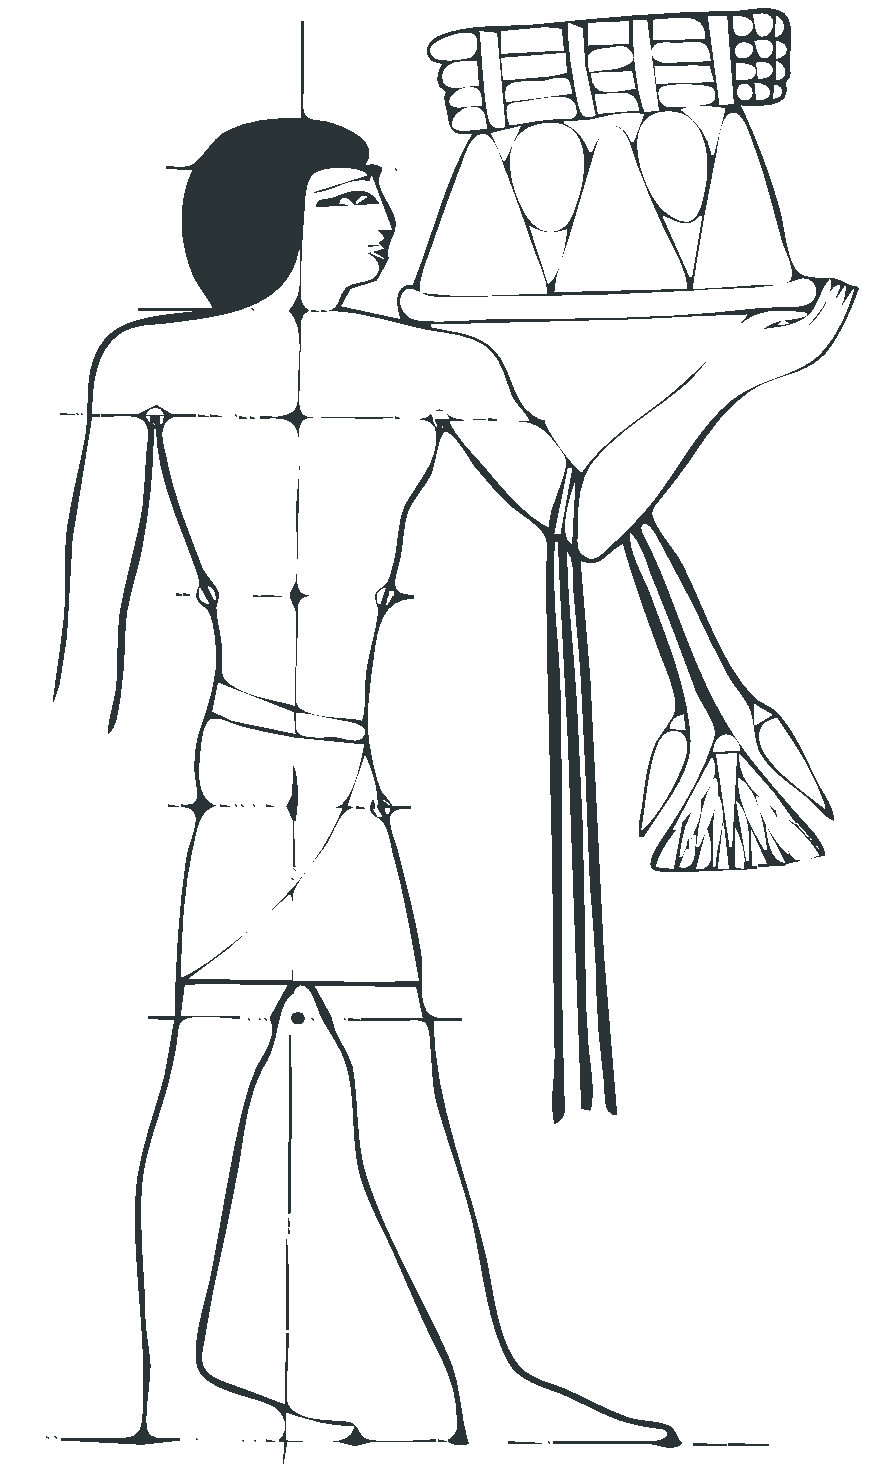
\includegraphics[width=.35\textwidth]{./images/egizi_canone_piede.pdf}
% egizi_canone_piede.pdf: 421x708 pixel, 72dpi, 14.85x24.98 cm, bb=0 0 421 708
\caption{Uno dei primi canoni egizi.}
\label{fig:egyptian_canon}
\end{figure}

Diverse illustrazioni di arte Egizia mostrano anche come i tre riquadri superiori del canone venissero divisi a loro volta in cinque parti ognuno, per poter disegnare il volto con più dettagli.

Le arti classiche dei Greci, per creare immagini della figura umana, rifiutarono il rigido sistema Egizio, che non era adatto a rappresentarne i movimenti. I Greci concepivano infatti l'arte come rappresentazione di un essere vivo, in contrasto agli Egizi, che cercavano di cristallizzare la figura umana per l'eternità.

Nell'iconometria Indiana, l'altezza facciale era utilizzata come modulo base dai due sistemi proporzionali, Śāriputra e Ālekhyalakṣaṇa, che riflettevano accuratamente le relazioni naturali delle diverse parti del corpo tra di loro. Il sistema Śāriputra, datato 1200 d.C., è conosciuto per le sculture in onore di Buddha (fig.~\vref{fig:sariputra_buddha}).

\begin{SCfigure}[][!ht]
\centering
\subfloat[][]
   {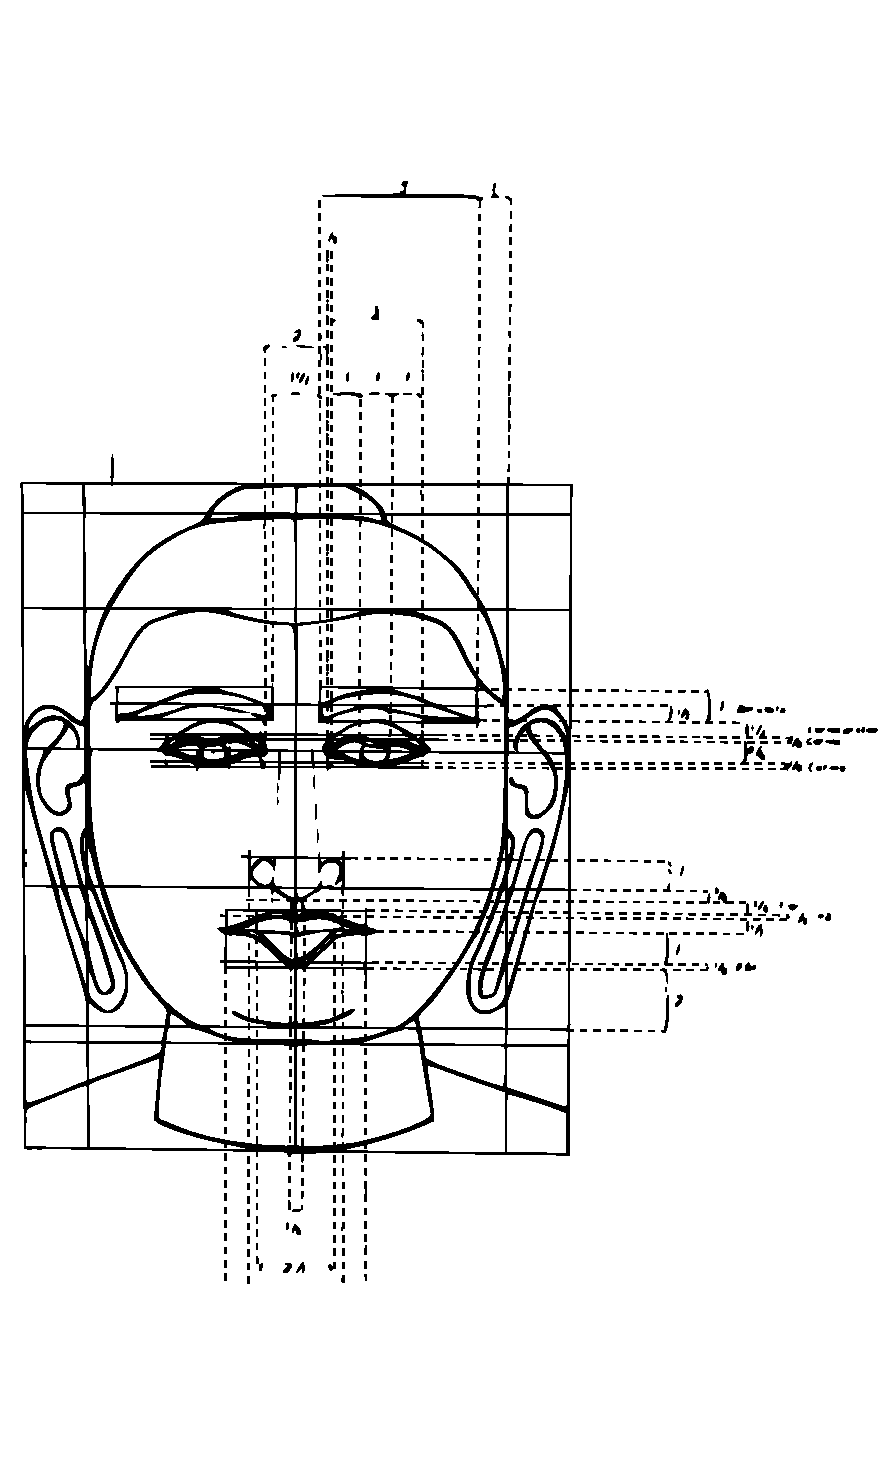
\includegraphics[width=.35\textwidth]{./images/sariputra_buddha_front.pdf}} \quad
\subfloat[][]
   {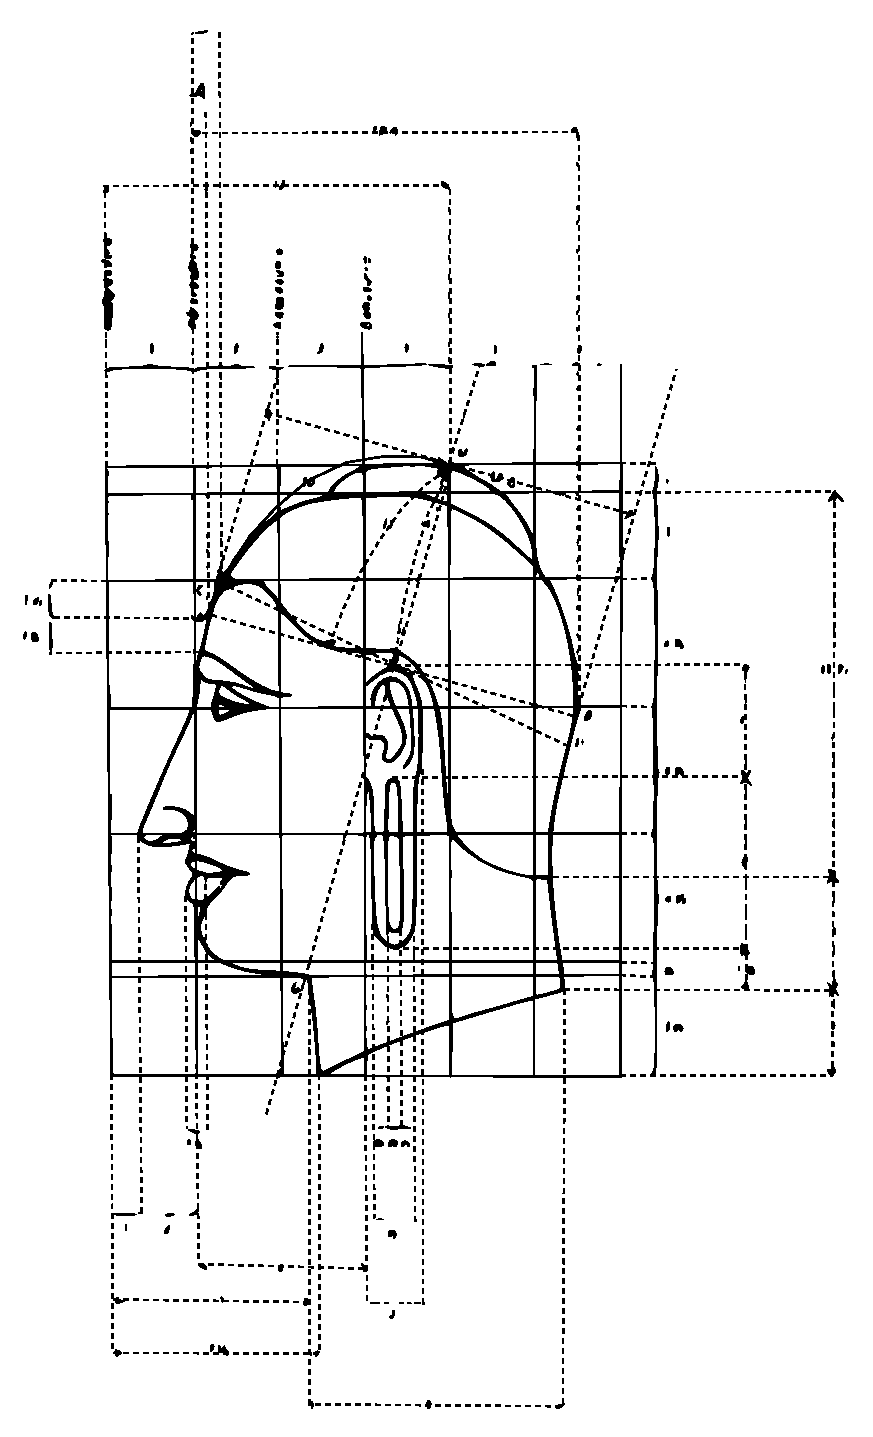
\includegraphics[width=.35\textwidth]{./images/sariputra_buddha_side.pdf}}
\caption{Visione frontale (a) e laterale (b) di una statua del Buddha, secondo il sistema proporzionale Śāriputra.}
\label{fig:sariputra_buddha}
\end{SCfigure}

\begin{wrapfigure}{L}{.45\textwidth}
 \centering
 
\includegraphics[width=.4\textwidth]{./images/byzantin_canon.pdf}
 \caption{Sistema a tre cerchi concentrici nell'arte Bizantina.}
 \label{fig:byzantin_canon}
\end{wrapfigure}

Nell'impero Bizantino, la griglia rettangolare del canone venne sostituita da uno schema di tre cerchi concentrici, con la lunghezza del naso come raggio per disegnare i due cerchi successivi. Il cerchio interno delineava la fronte e gli zigomi; il secondo cerchio, con un raggio pari a due volte il naso, definiva le misure esterne della testa, inclusi i capelli e il limite inferiore del volto. Il cerchio più esterno attraversava il giugulo e formava l'aureola.

\section{Dal Rinascimento al ventesimo secolo}
Lo sconvolgimento che il quindicesimo secolo portò nel pensiero artistico, nei concetti e nella tecnica è esemplificato dalle opere di Leonardo da Vinci (1459--1519) e Albrecht Dürer (1471--1528). Il lascito di Leonardo come esponente del Rinascimento va ben oltre l'Ultima Cena e la Monna Lisa. I suoi disegni includono infatti studi sulle proporzioni facciali, e la proiezione di un sistema di coordinate sul volto di un ``uomo a cavallo''.

\begin{figure}[!th]
\centering
\subfloat[][]
   {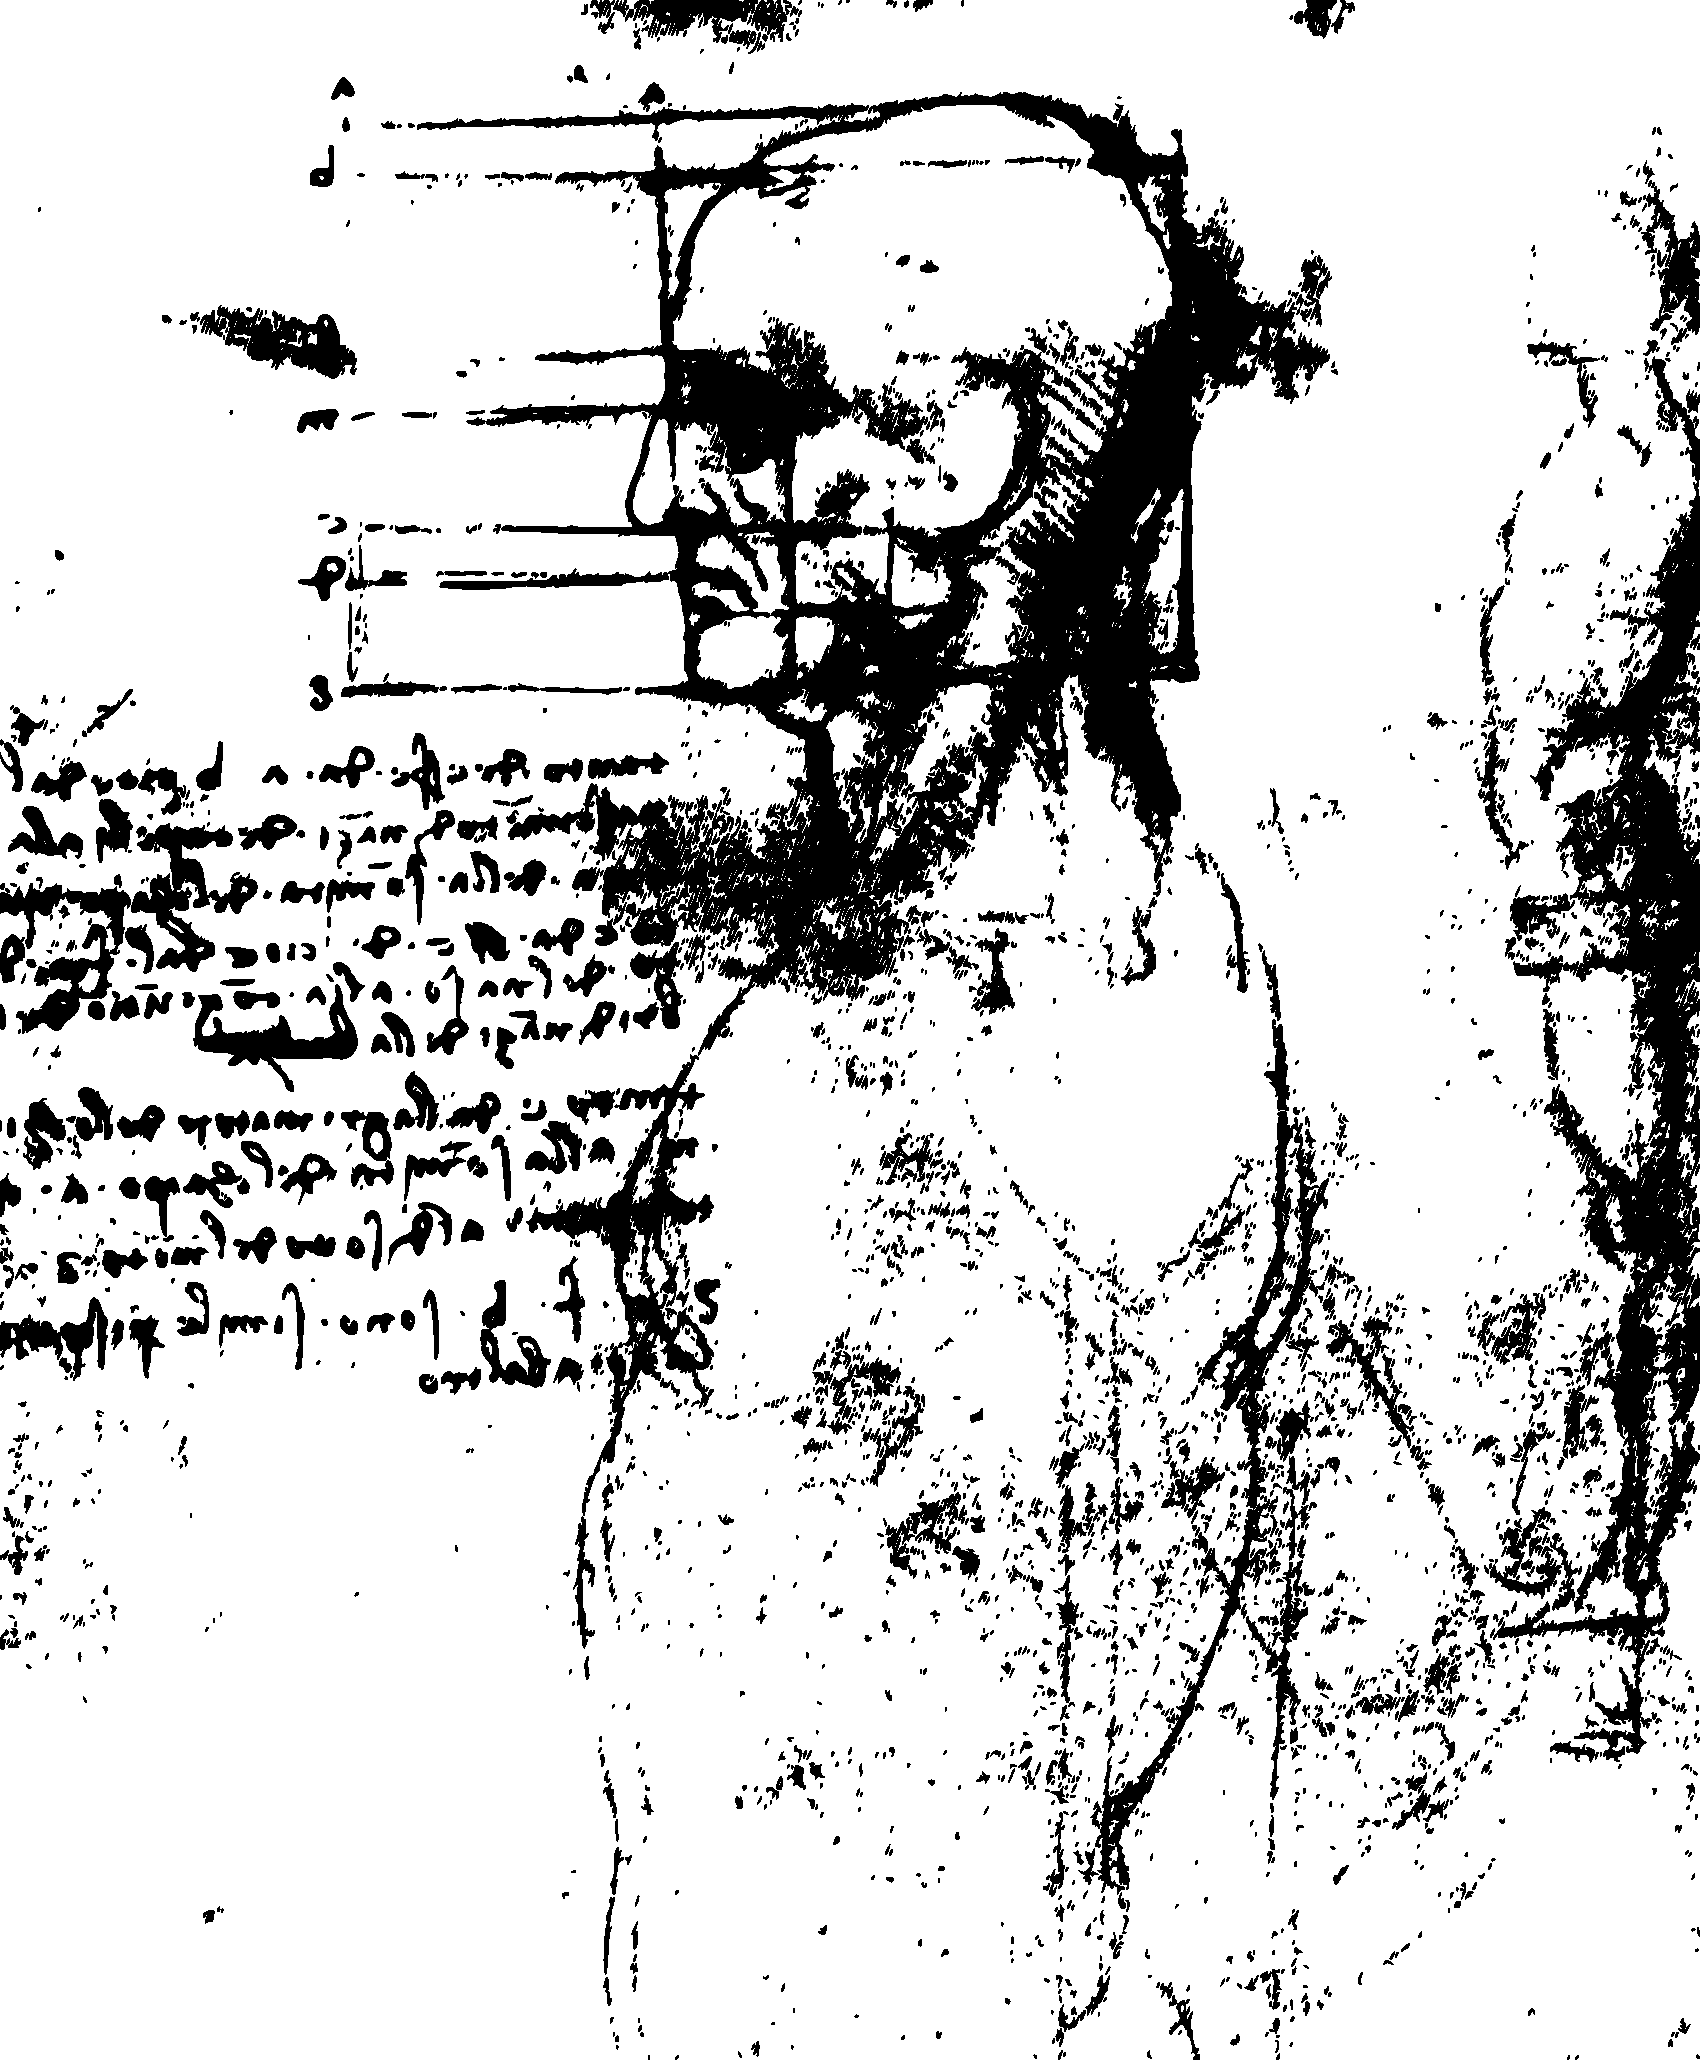
\includegraphics[width=.4\textwidth]{./images/leonardo1.pdf}} \quad
\subfloat[][]
   {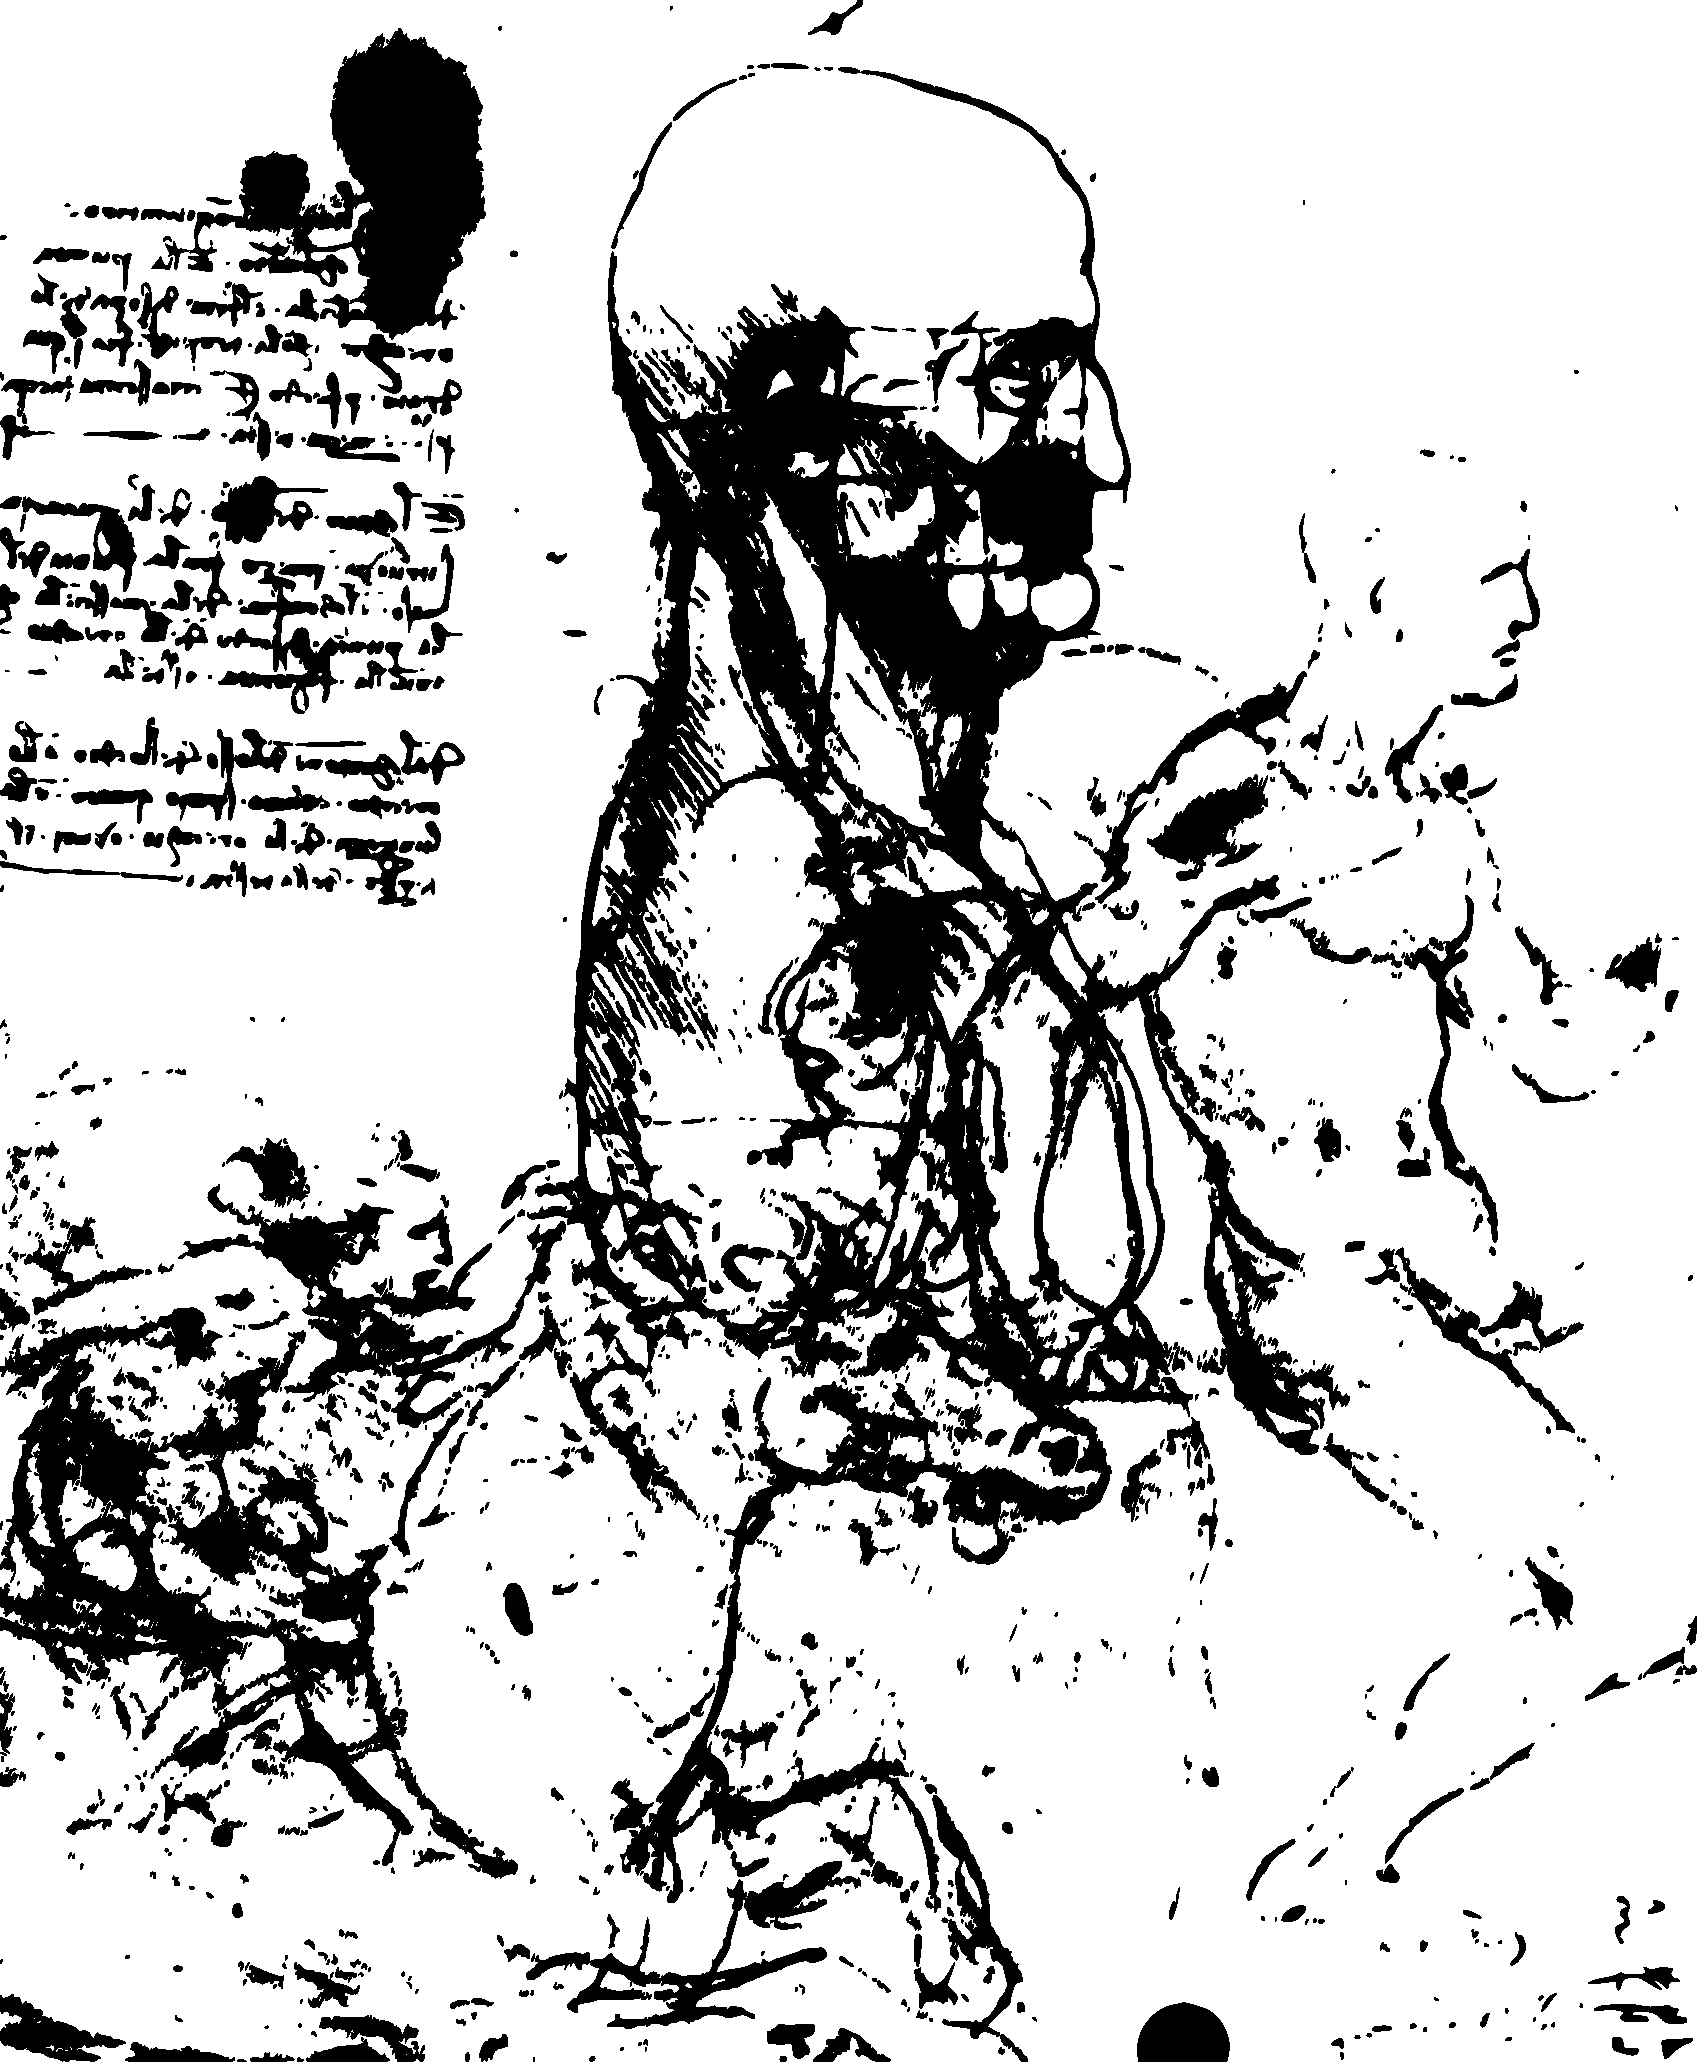
\includegraphics[width=.4\textwidth]{./images/leonardo2.pdf}}
\caption{Studi sul cranio e sul volto effettuati da Leonardo da Vinci.}
\label{fig:leonardo}
\end{figure}

\begin{SCfigure}[][!th]
\centering
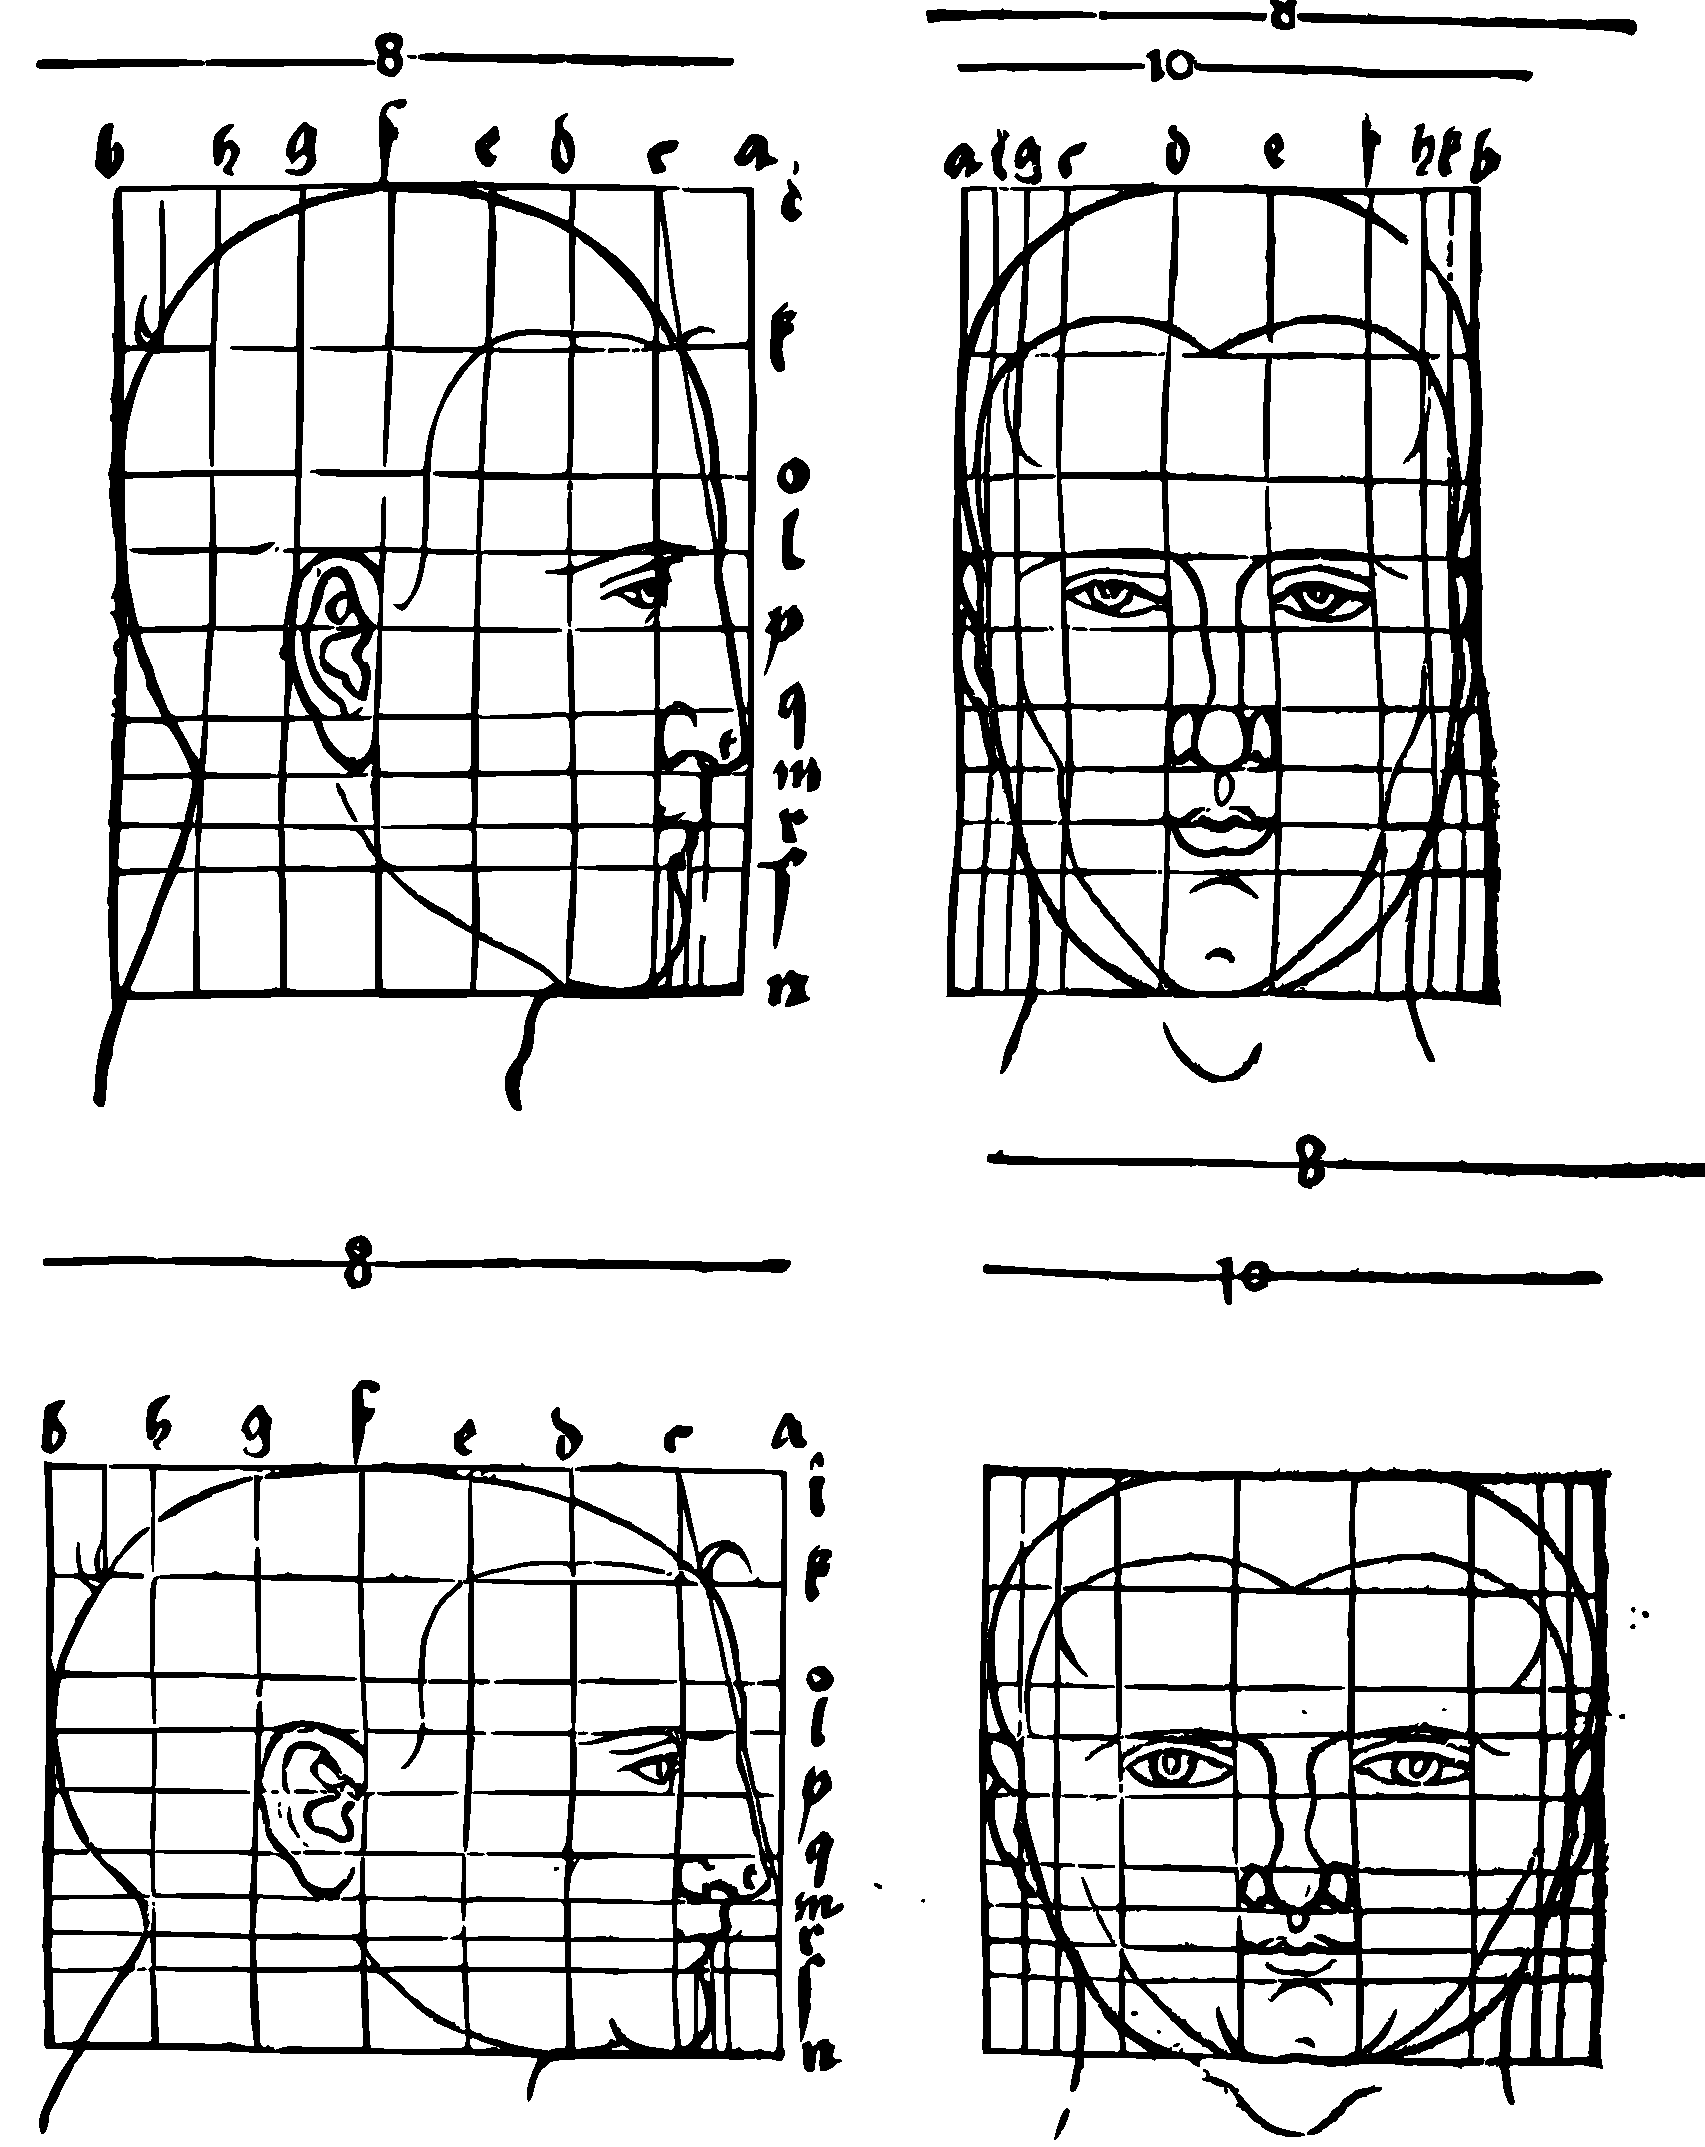
\includegraphics[width=.4\textwidth]{./images/duerer-proportional.pdf}
\caption{Analisi proporzionale di Dürer di un volto leptoprosopico ed uno euriprosopico.}
\label{fig:duerer}
\end{SCfigure}

Gli elaborati studi di Albrecht Dürer sulla prospettiva delle proporzioni umane sono ineguagliati ad oggi; infatti, i quattro libri di Dürer sulle proporzioni ``segnano un climax che la teoria delle proporzioni non ha mai raggiunto prima o avrebbe mai potuto raggiungere dopo''\footcite{Panofsky1974}.

Usando metodi strettamente geometrici, Dürer fornì un'analisi proporzionale dei volti leptoprosopici (stretti e lunghi) e dei volti euriprosopici (larghi e corti) in un sistema di coordinate in cui le linee orizzontali e verticali erano disegnate passanti per gli stessi punti facciali (fig.~\vref{fig:duerer}).

\begin{wrapfigure}{R}{.4\textwidth}
\centering
\fbox{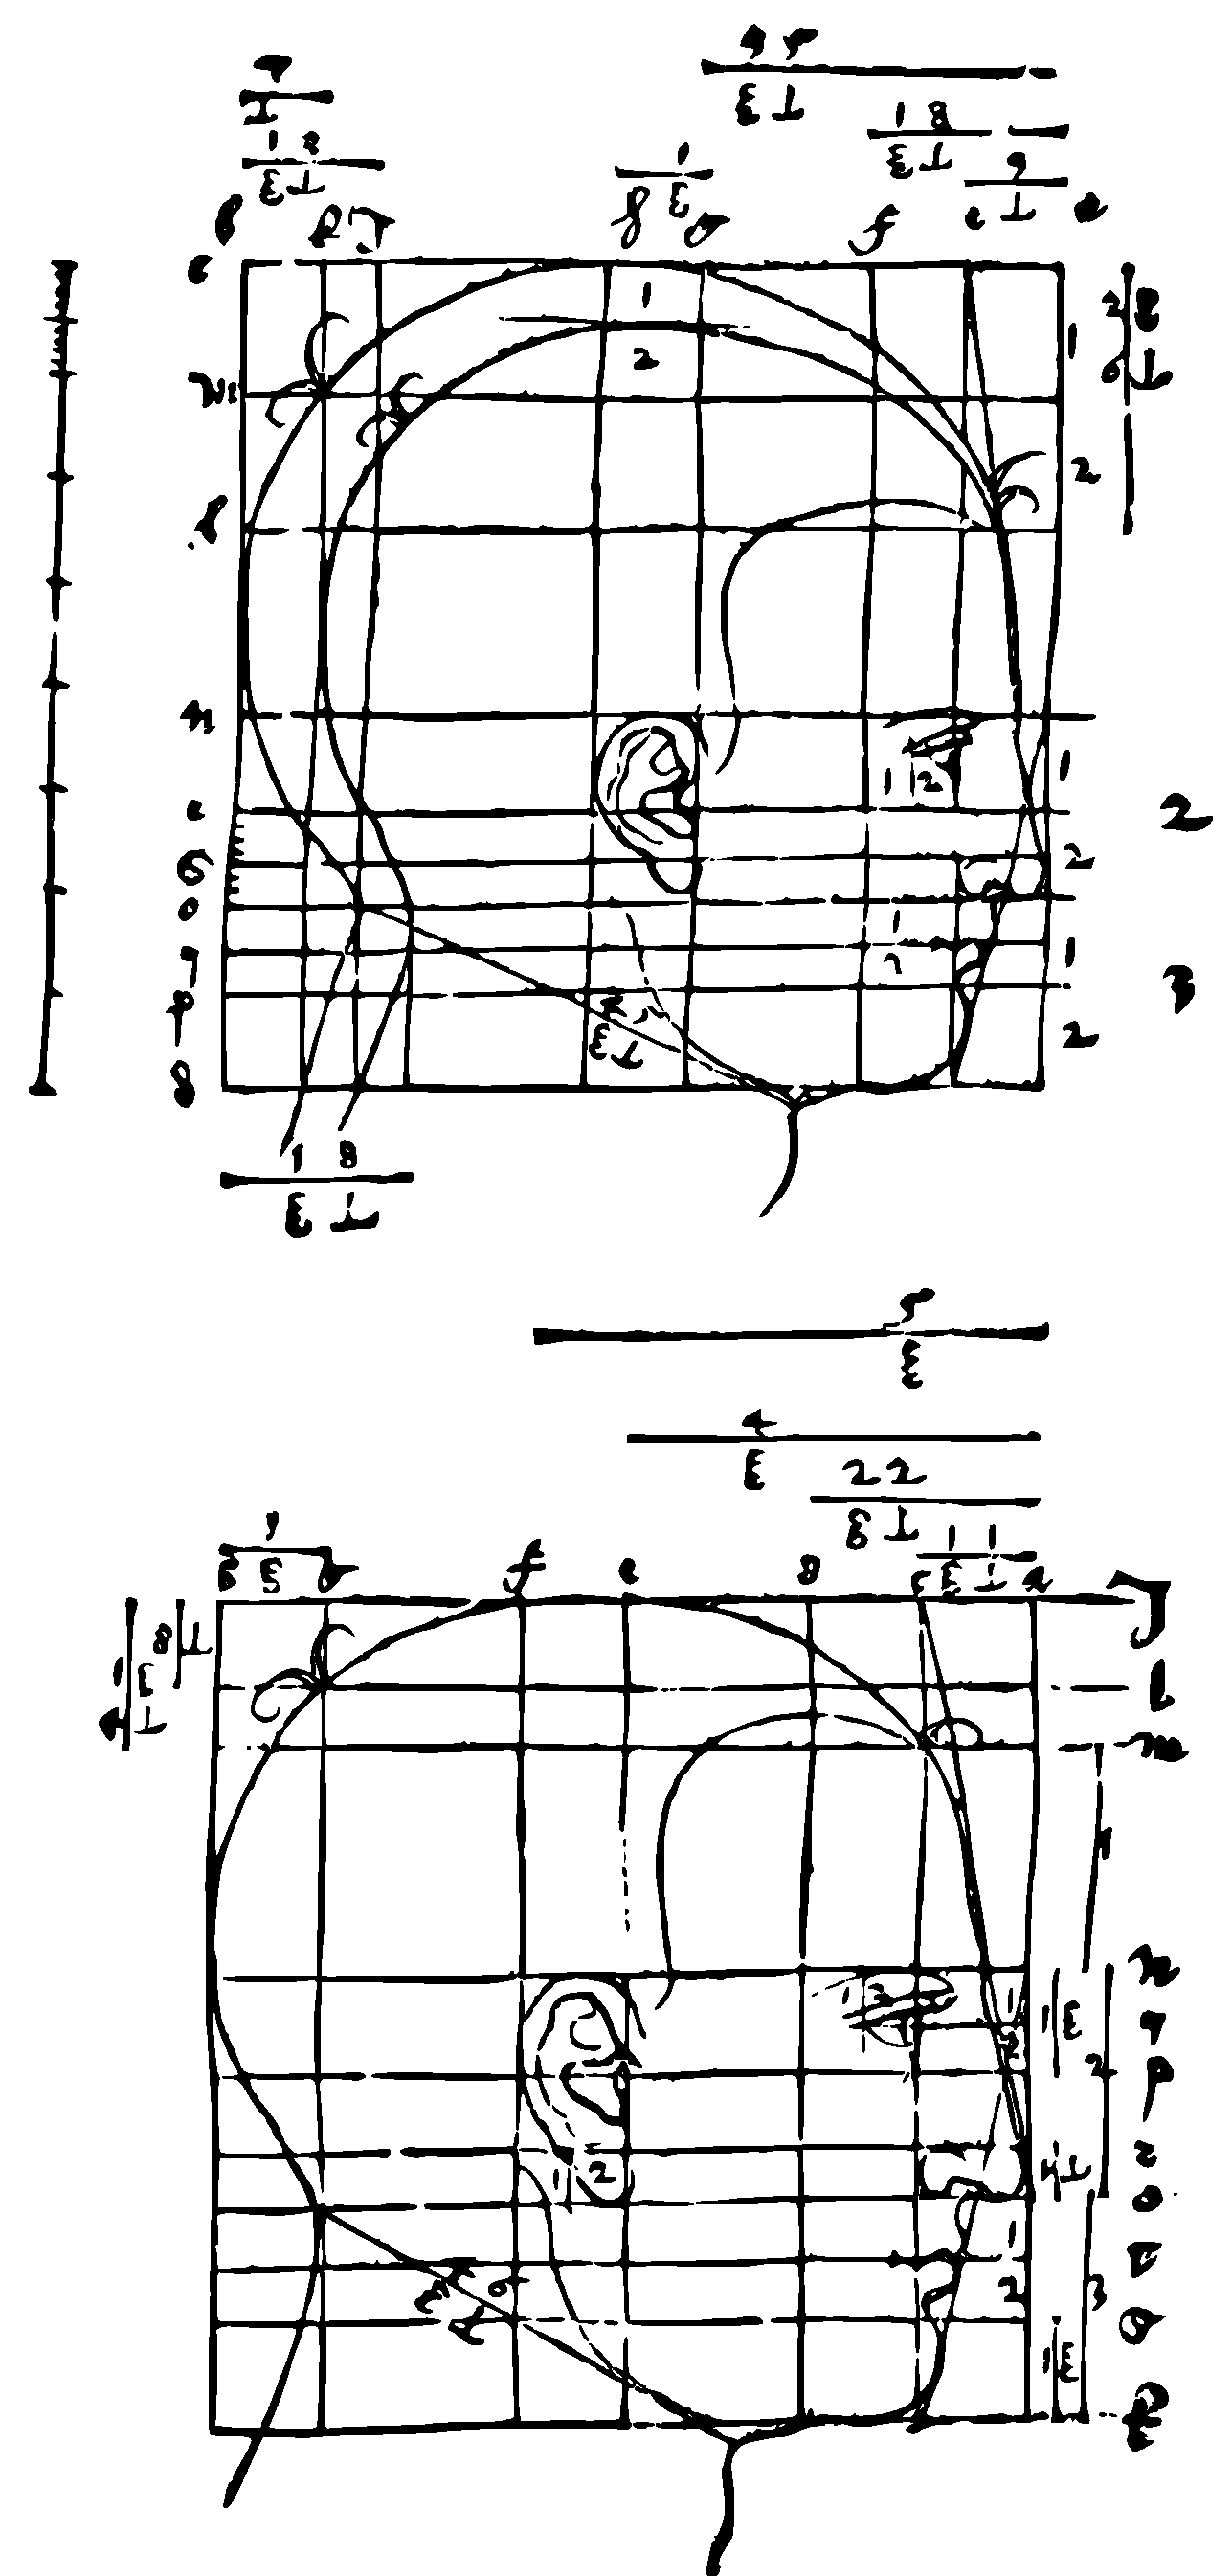
\includegraphics[width=.35\textwidth]{./images/duerer-proportional-2.pdf}}
\caption{Influenza dell'angolo facciale sul profilo secondo Dürer.}
\label{fig:duerer2}
\end{wrapfigure}

In aggiunta al sistema di coordinate, Dürer fece uso di due linee -- una disegnata dalla fronte tangente al naso, l'altra tangente al mento e al labbro superiore -- che insieme creavano un'area triangolare che caratterizzava il profilo facciale attraverso un ``angolo facciale'' (fig.~\vref{fig:duerer2}).

I disegni di Dürer attestano i continui sforzi nel definire le variazioni della morfologia facciale. Uno di questi è particolarmente significativo, e rappresenta un punto chiave dell'evoluzione dell'analisi cefalometrica così come è conosciuta oggi. In esso, la differenza tra un profilo facciale retruso e uno protruso è mostrato da un cambiamento dell'angolo tra gli assi verticali e orizzontali di un sistema di coordinate caratterizzante la configurazione facciale di ogni soggetto. Perciò un singolo angolo diventa l'espressione della differenza nella morfologia facciale tra due individui.

\begin{figure}[!ht]
 \centering
 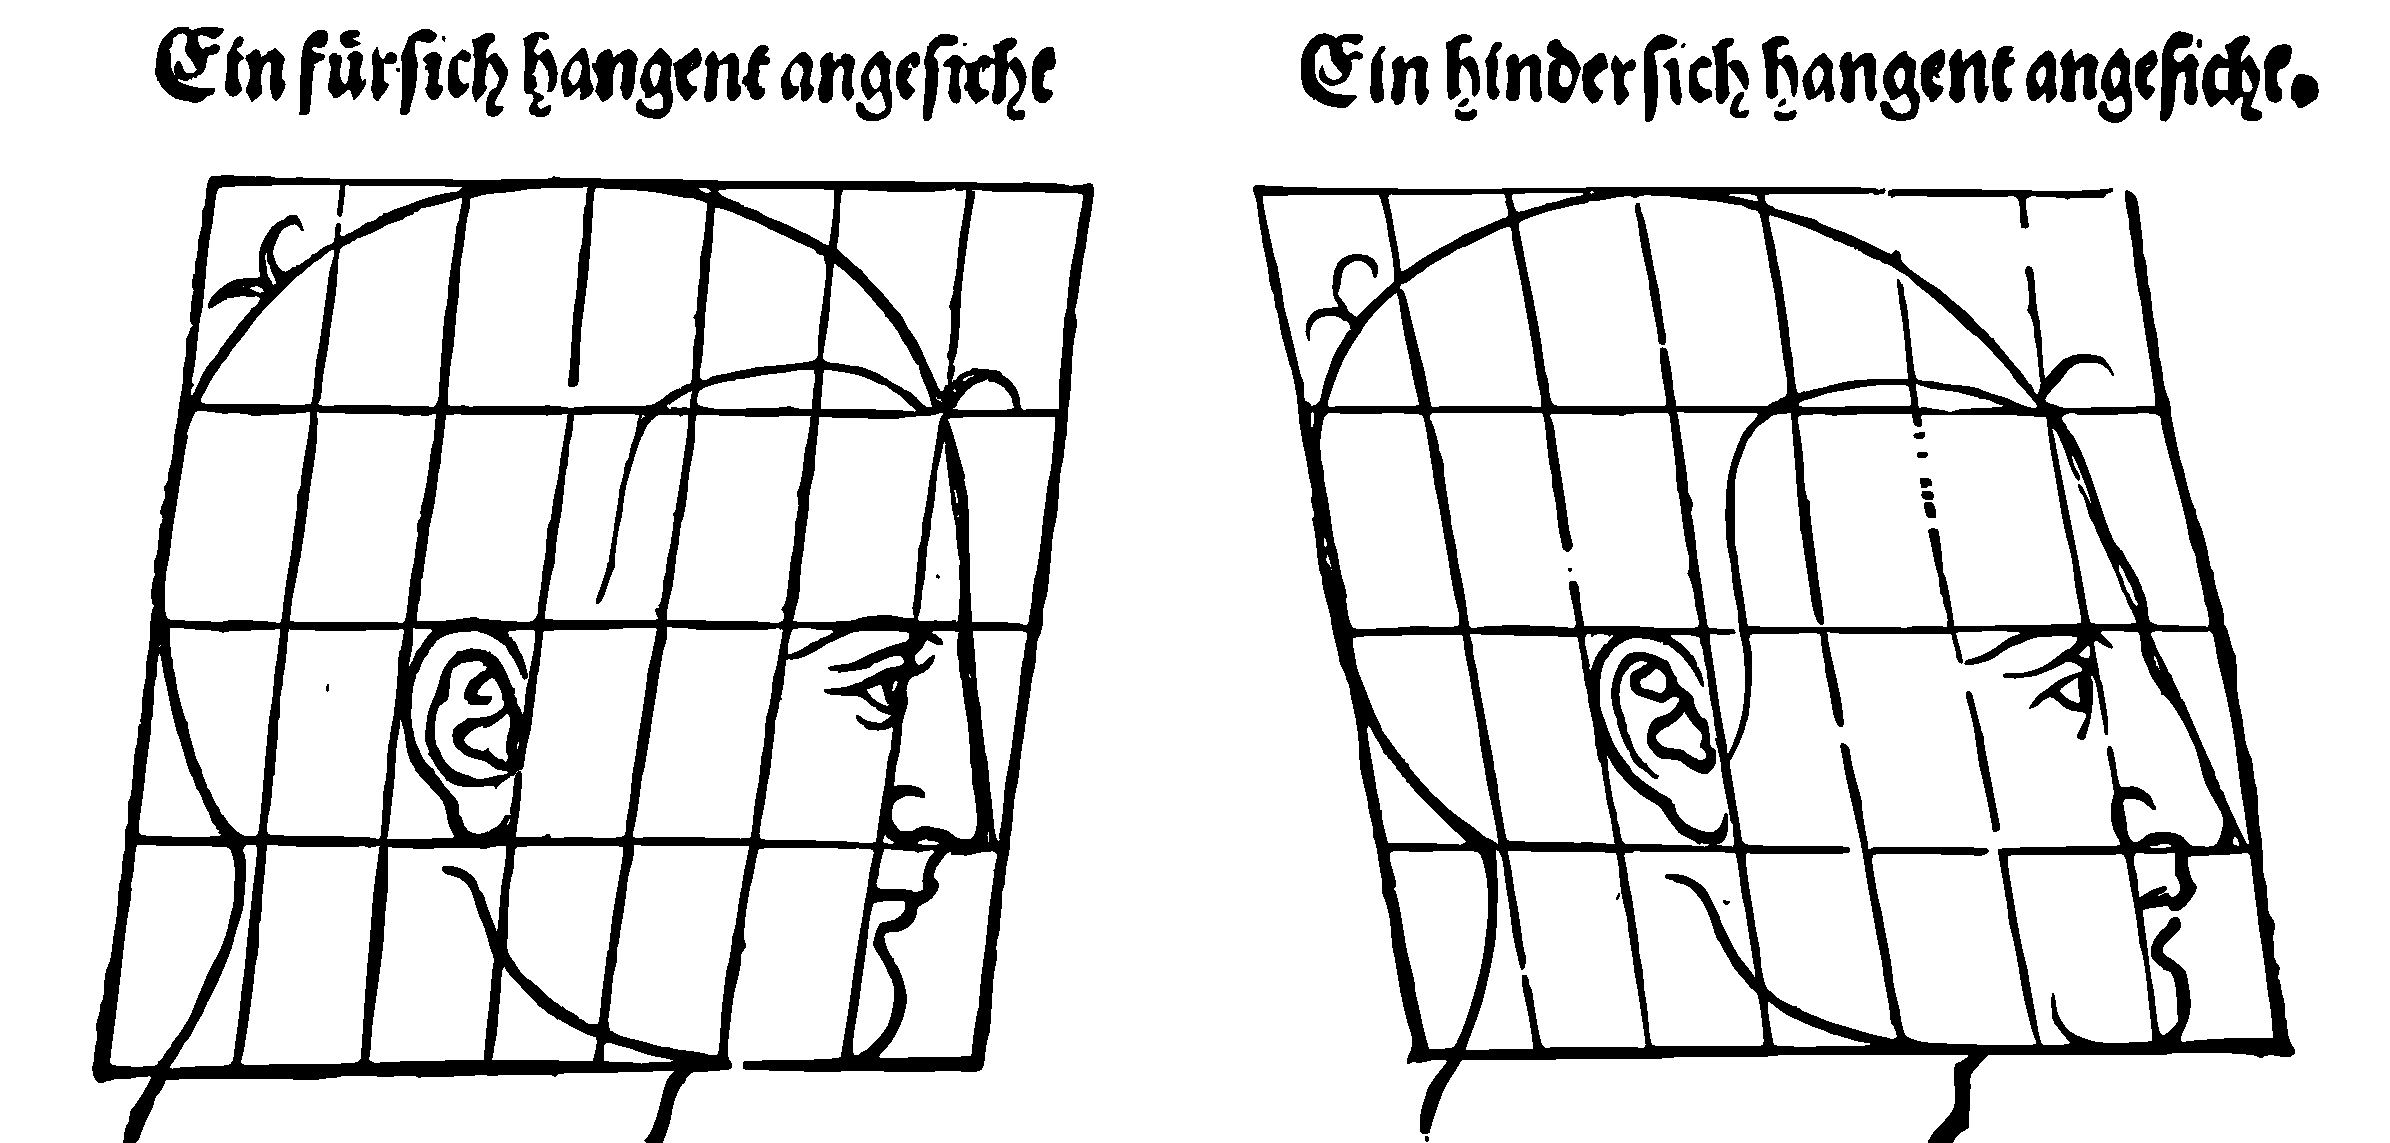
\includegraphics[width=.5\textwidth]{./images/duerer-proportional-3.pdf}
 % duerer-proportional-3.jpg: 1434x686 pixel, 72dpi, 50.59x24.20 cm, bb=0 0 1434 686
 \caption{Variazione del profilo conseguente una variazione degli angoli}
 \label{fig:duerer3}
\end{figure}

Petrus Camper (1722--1789) fu un medico e scienziato che effettuò ampi studi sui crani. Il successo dei suoi studi si basava sull'orientamento dei crani nello spazio su un piano orizzontale, passante per il meato acustico esterno e un punto al di sotto del naso. Questi punti non erano rigorosamente definiti, ma Camper veniva guidato dalla direzione del processo zigomatico. In molte delle sue illustrazioni, questo piano orizzontale veniva disegnato passante per la spina nasale anteriore.

Il \textit{piano di Camper} divenne un piano di riferimento per le misure angolari utilizzate per caratterizzare gli andamenti evolutivi negli studi di morfologia facciale e sull'in\-vec\-chi\-a\-men\-to. Questo piano viene ancora oggi utilizzato in protesi per stimare l'angolazione del piano occlusale nei pazienti edentuli, poiché è generalmente parallelo.

Egli vide come un singolo angolo descrivesse il profilo caratteristico di una faccia. Questa cambia nella sua totalità, ma l'angolo facciale è l'indice di una deformazione generale.

L'angolo facciale di Camper venne prontamente accettato come una misura standard nello studio del cranio. I termini \textit{prognatico} e \textit{ortognatico} sono legati alle illustrazioni di Camper della forma facciale negli uomini e nei primati. Come risultato, l'angolo tra il piano orizzontale e la linea Nasion-Prosthion divenne il metodo antropologico d'elezione per determinare il tipo facciale. Il termine \textit{prognatismo} si riferisce alla prominenza della mandibola rispetto alla fronte; \textit{ortognatismo} si riferisce invece ad  un profilo facciale piatto.

\begin{SCfigure}[][!ht]
 \centering
 \fbox{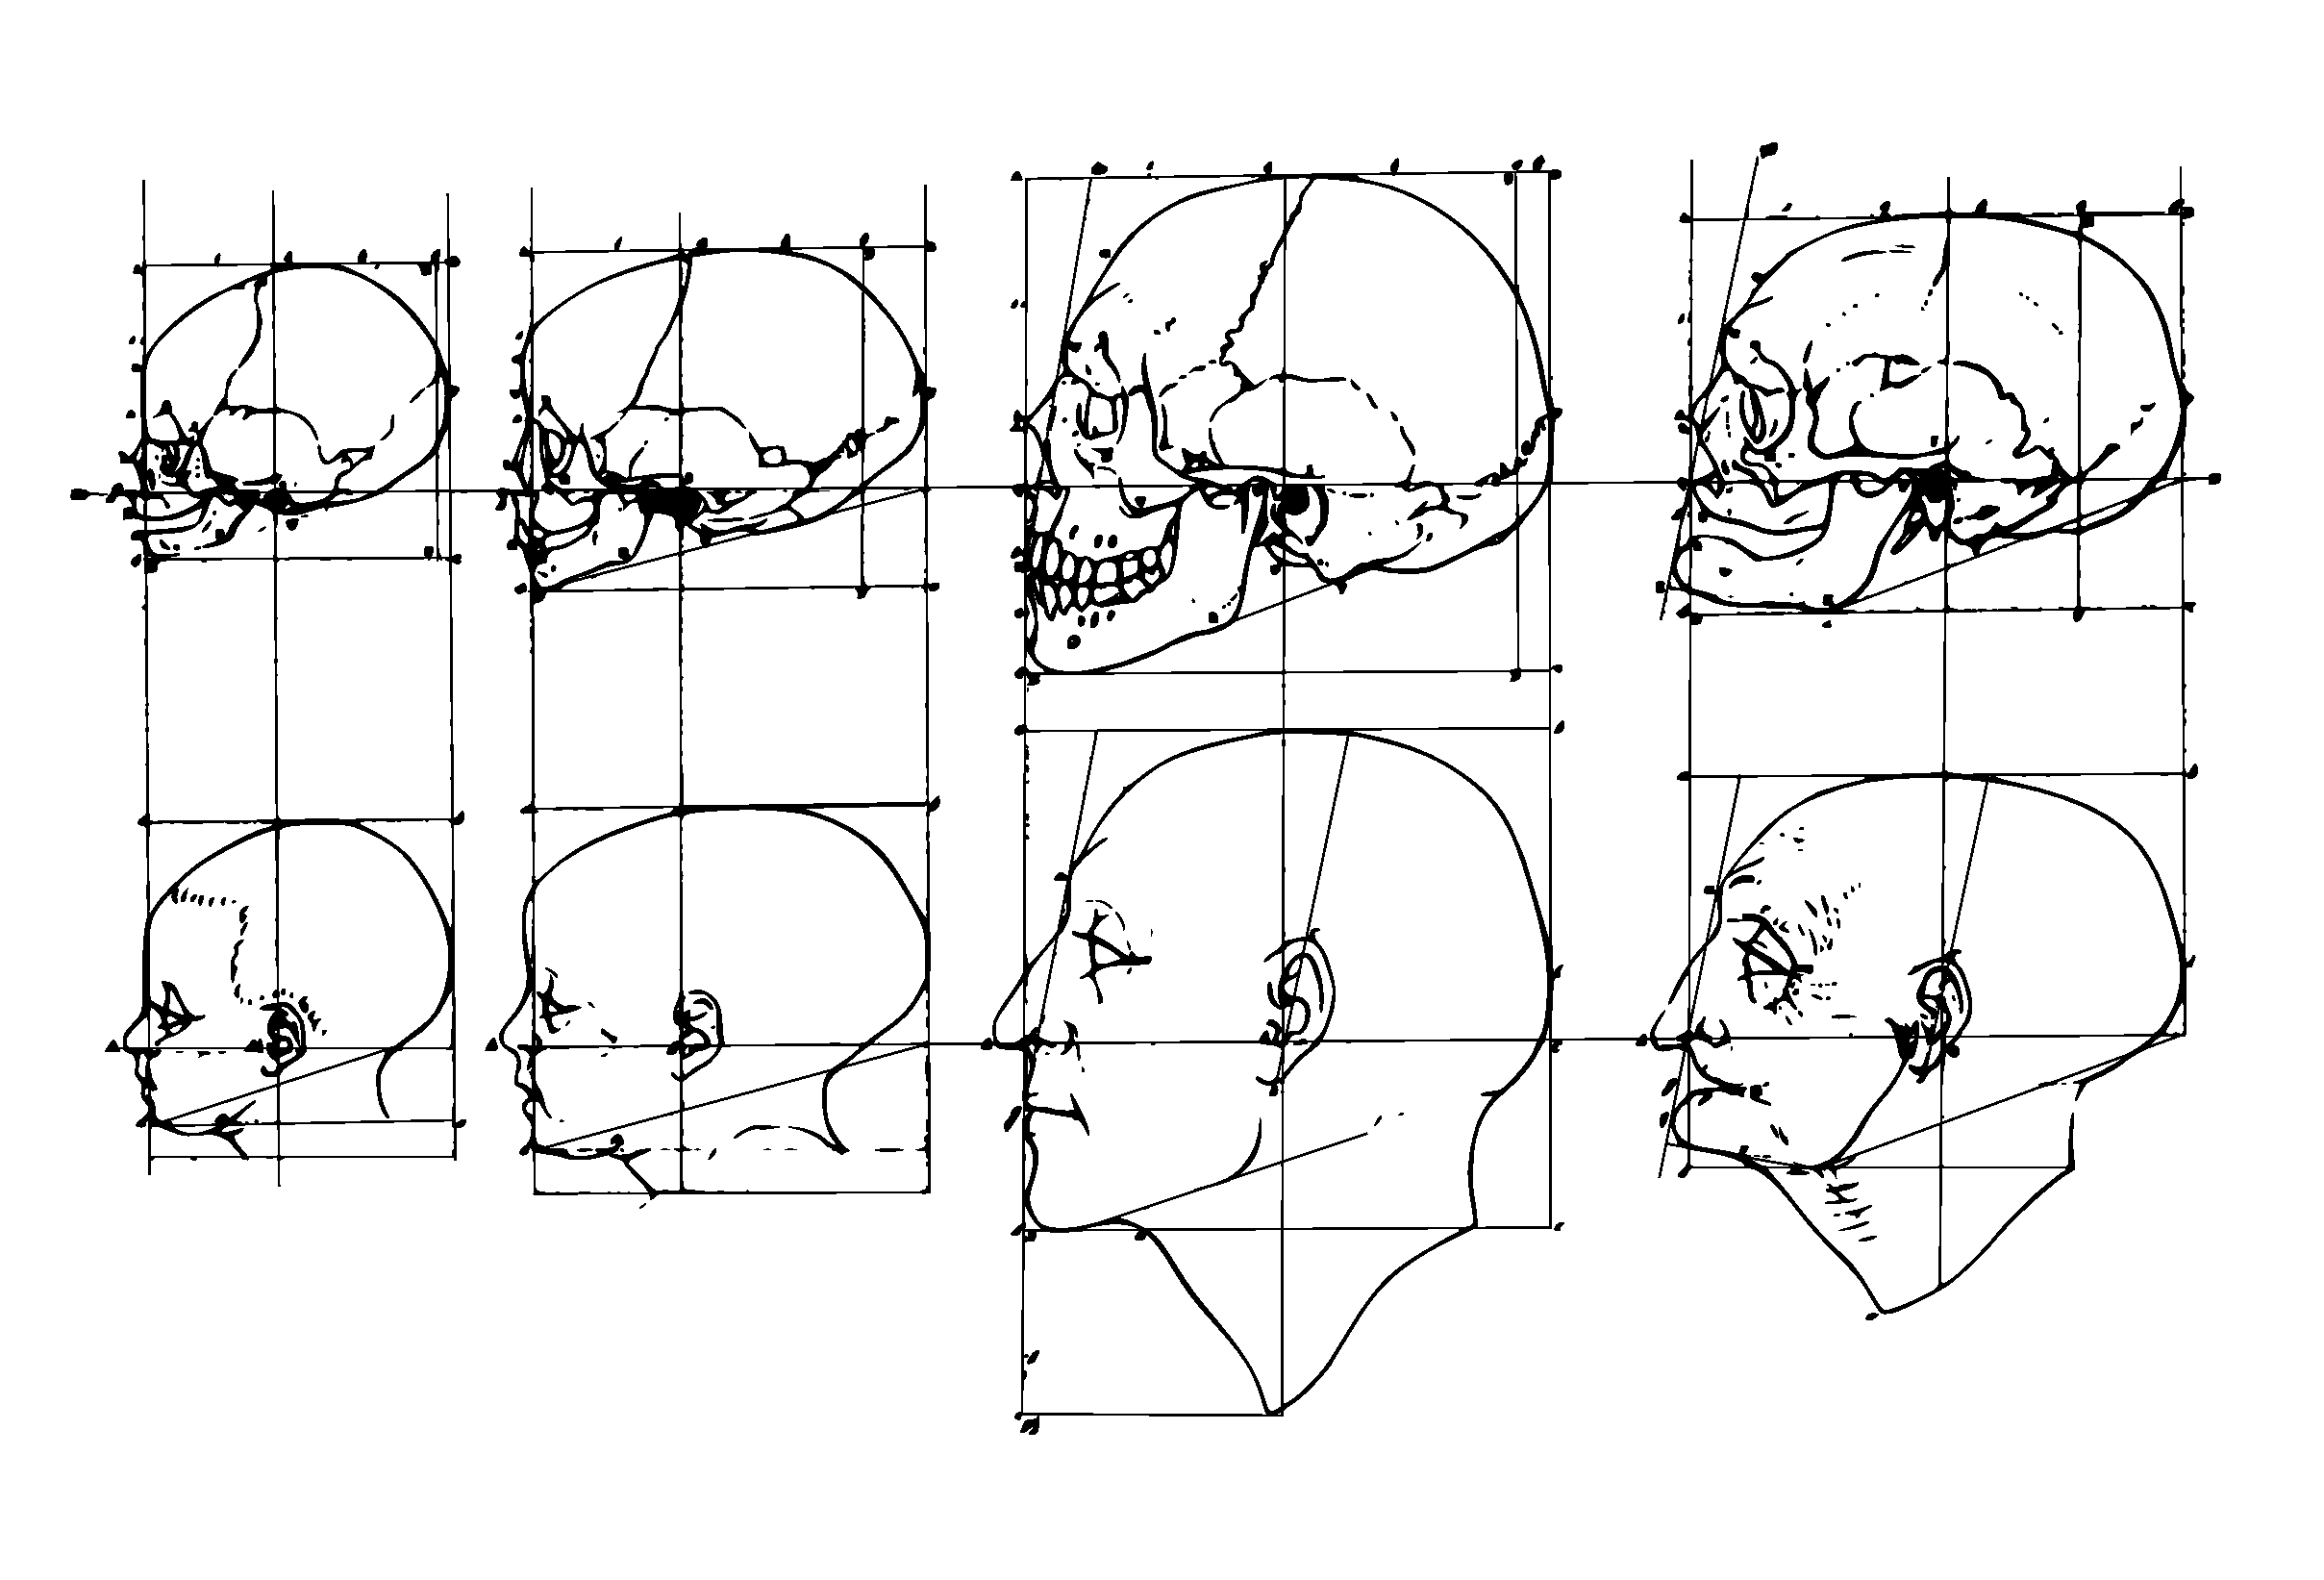
\includegraphics[width=.7\textwidth]{./images/camper-crani.pdf}}
 \caption{Studi di Camper sulle variazioni del cranio durante la crescita}
 \label{fig:camper-crescita}
\end{SCfigure}

\begin{wrapfigure}{R}{.45\textwidth}
 \centering
 \fbox{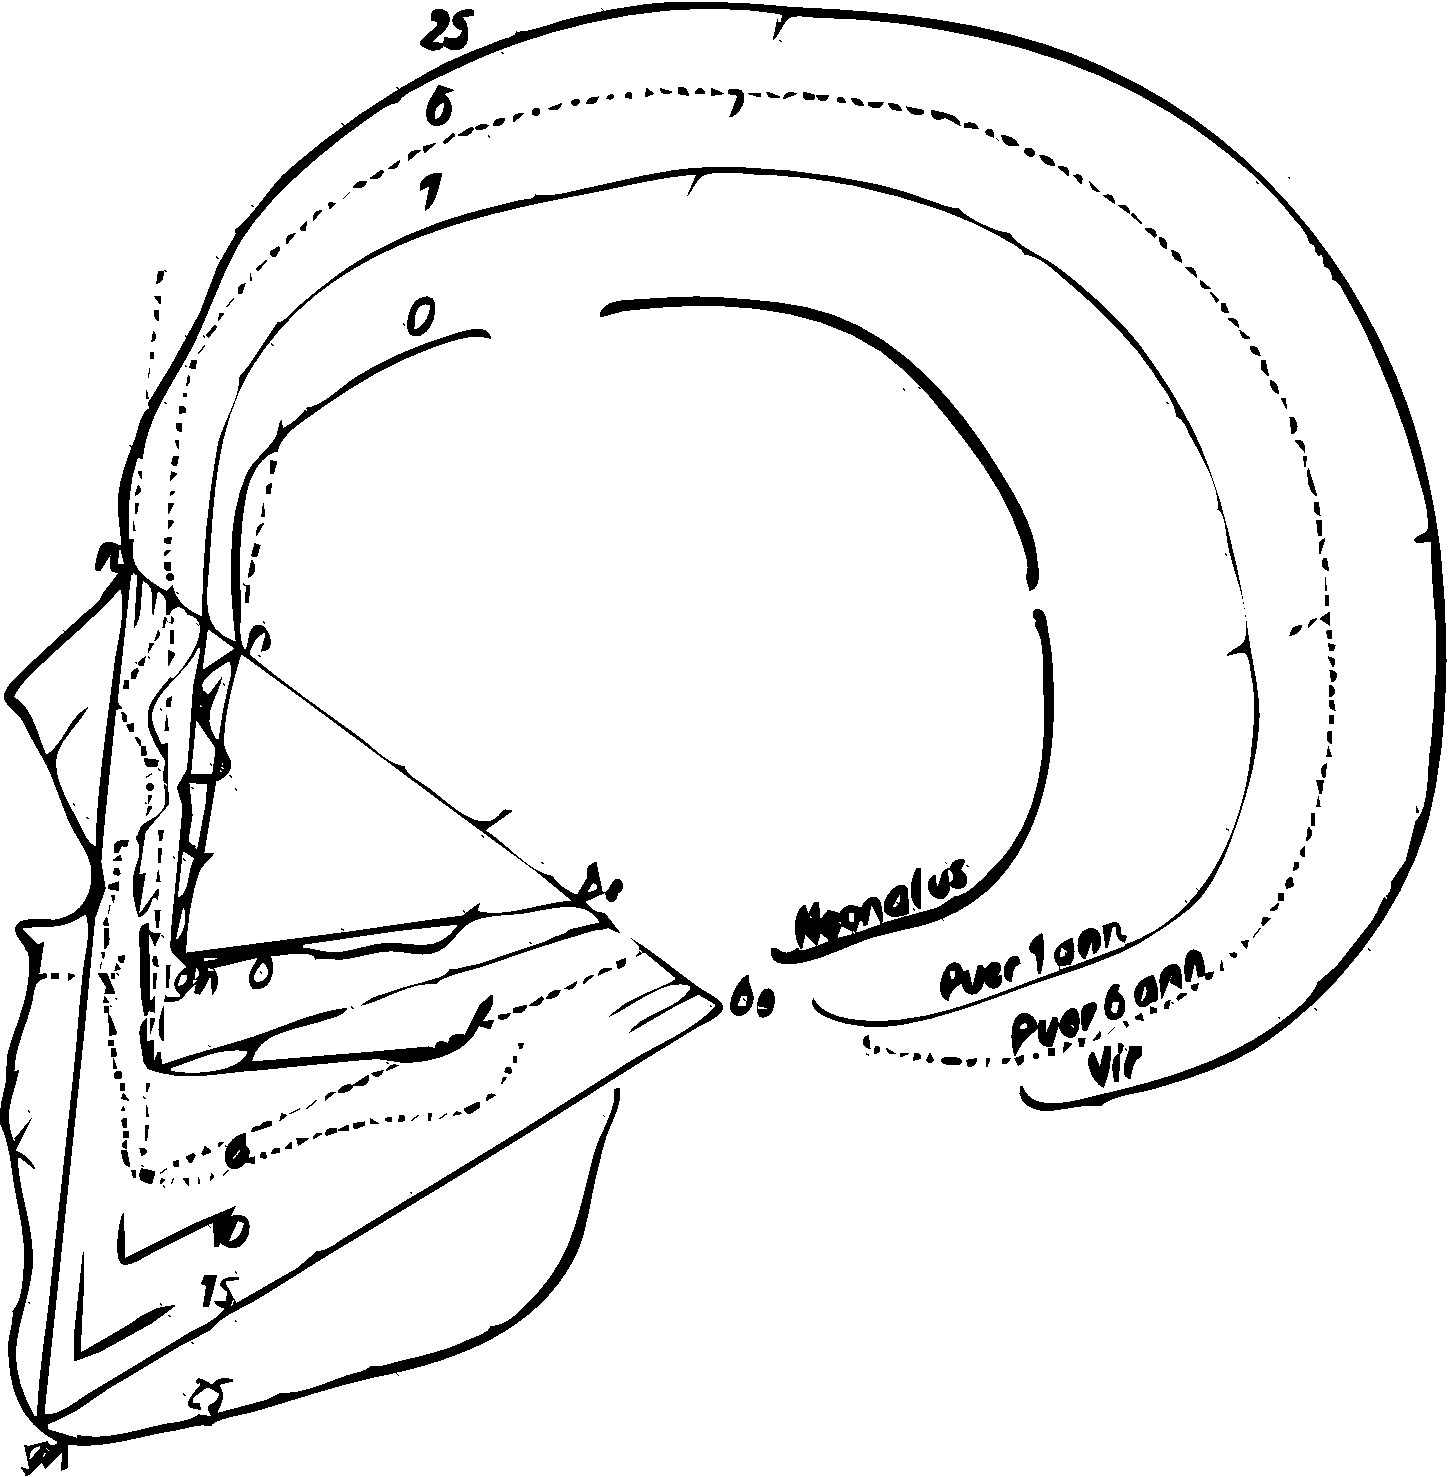
\includegraphics[width=.4\textwidth]{./images/welcker-growth.pdf}}
 % welcker-growth.pdf: 695x709 pixel, 72dpi, 24.52x25.01 cm, bb=0 0 695 709
 \caption{Crescita cranica secondo Welcker.}
 \label{fig:welcker}
\end{wrapfigure}

Camper studiò anche le differenze nella forma facciale legate al processo di invecchiamento (fig.~\vref{fig:camper-crescita}). La prima morfologia esaminata fu quella di un neonato, seguita da quella di un bambino di circa 8 anni, un adulto e un anziano. I cambiamenti vennero analizzati tenendo fisso il piano orizzontale, e consistono in una crescita della parte inferiore del volto fino all'età adulta, e il suo successivo accorciamento con la perdita progressiva di tutti i denti.

Gli studi di Welcker (1862) sulla crescita e lo sviluppo del cranio umano, dimostrarono la discesa e rotazione della mandibola durante l'ontogenesi, attraverso una configurazione triangolare dal Basion al Gnathion (fig.~\vref{fig:welcker})\footcite{Welcker1866}. Questo schema triangolare fu successivamente modificato in un poligono da Hellman (fig.~\vref{fig:hellman})\footcite{Hellman1935} per rappresentare la crescita facciale e per esaminare le differenze tra individui con malocclusioni di Classe II e Classe III. Dopo Hellman, questo poligono fu usato da Korkhaus\footcite{Korkhaus1939} e da Björk\footcite{Bjoerk1947} (fig.~\vref{fig:bjork-profili}). Quest'ultimo sviluppò questo poligono in quella che può essere definita l'analisi ``forma-spazio'' dello scheletro facciale; analisi che illustrò chiaramente la configurazione facciale dalla base cranica al piano mandibolare, e dall'articolazione temporomandibolare al profilo facciale.

\begin{SCfigure}[][!ht]
\centering
\fbox{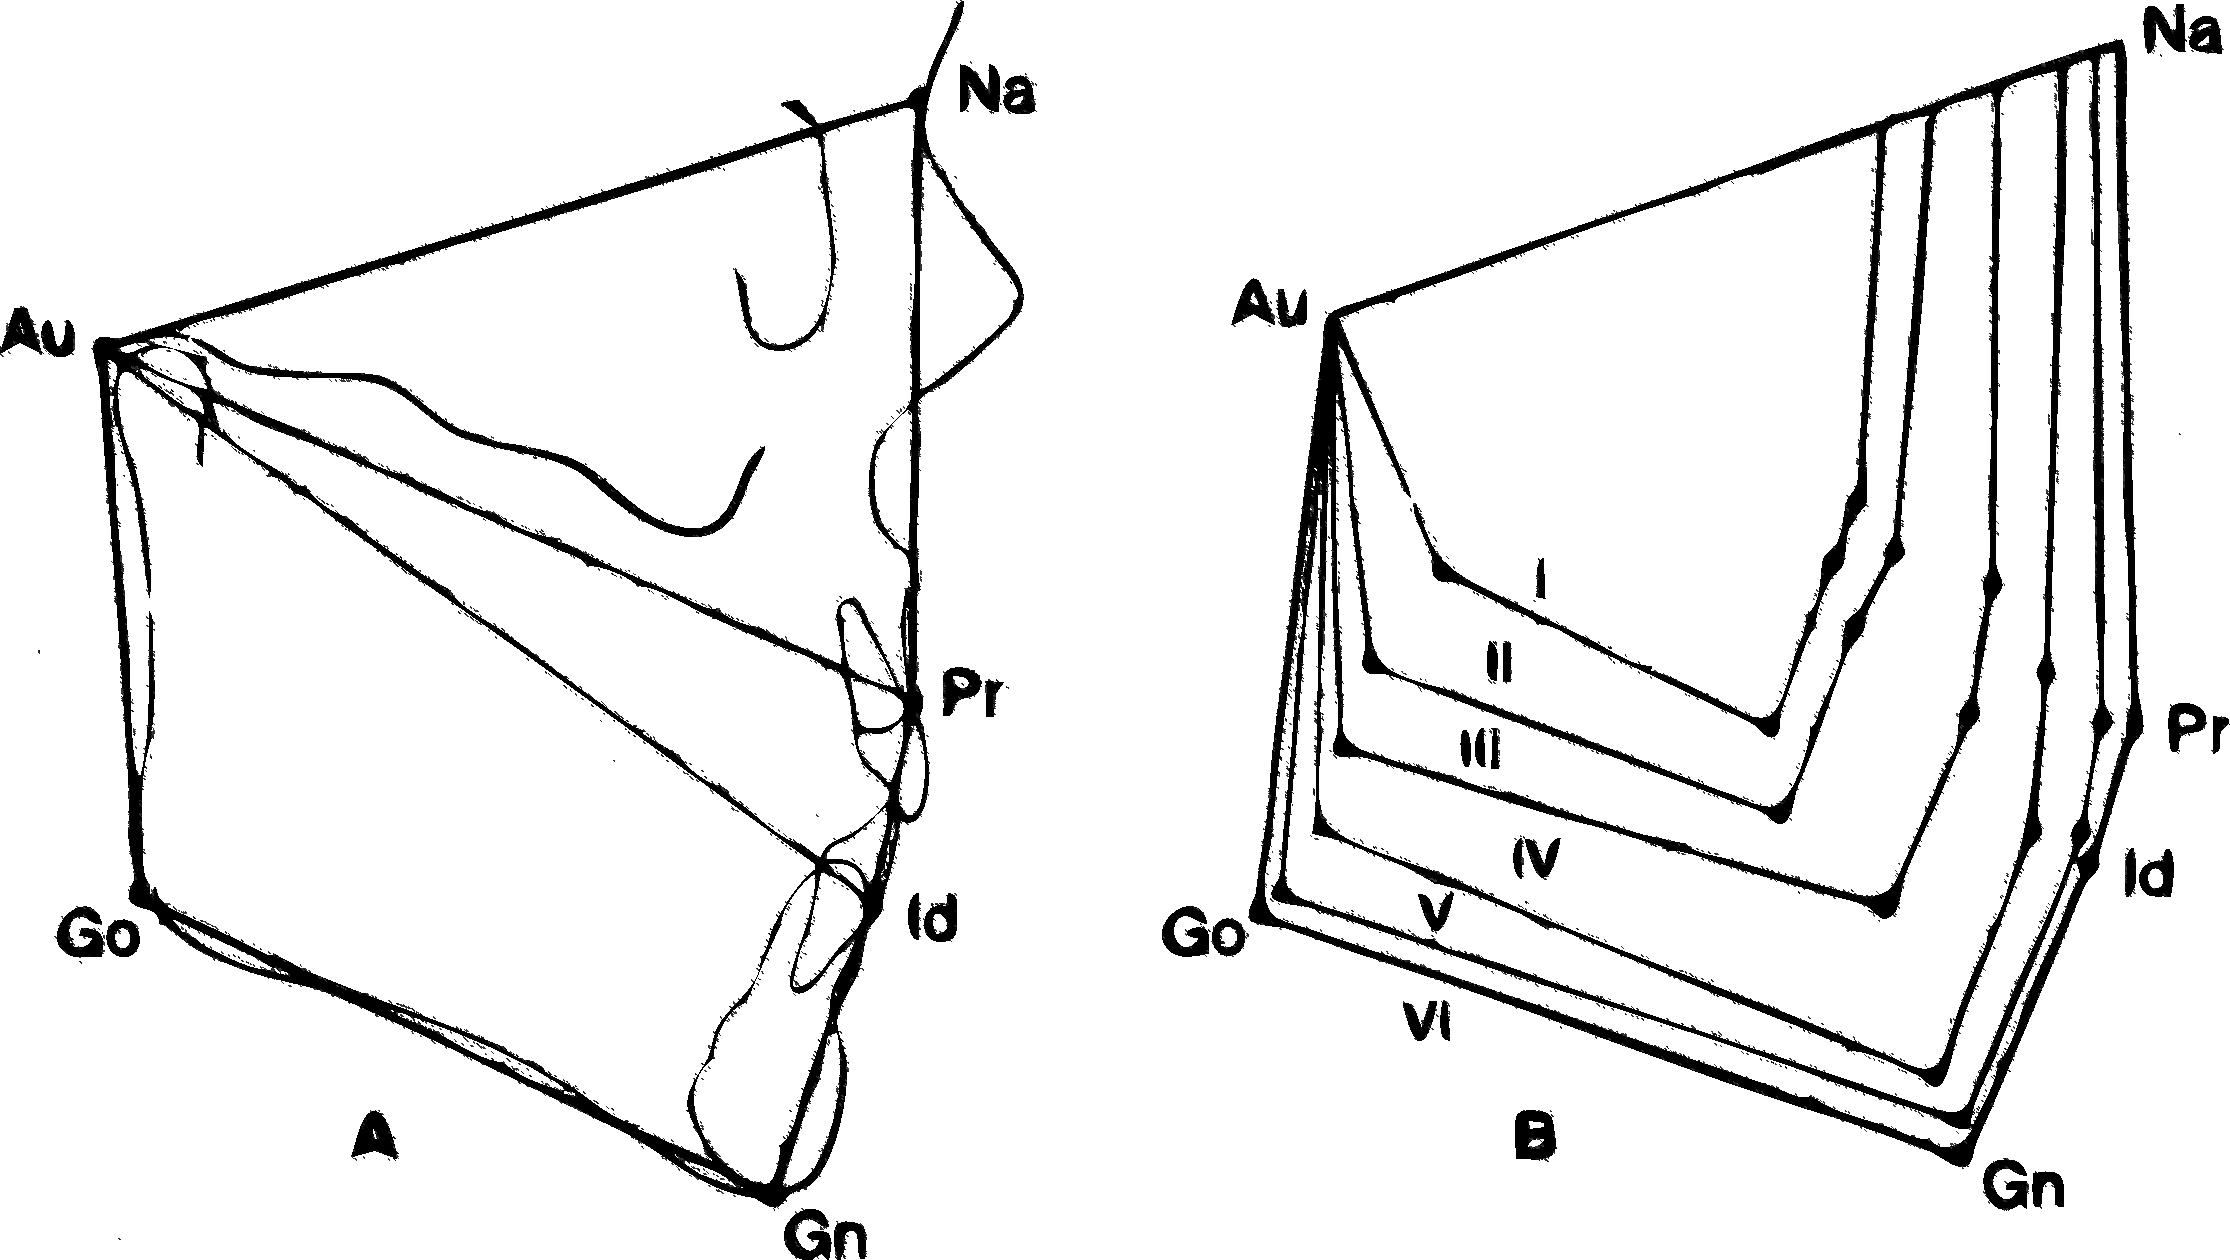
\includegraphics[width=.7\textwidth]{./images/hellman-growth.pdf}}
% hellman-growth.pdf: 1070x605 pixel, 72dpi, 37.75x21.34 cm, bb=0 0 1070 605
\caption{Analisi della crescita facciale proposta da Hellman, usando un poligono e la linea da Nasion ad Auricolare come riferimento.}
\label{fig:hellman}
\end{SCfigure}

\begin{figure}[!ht]
\centering
\subfloat[][]
   {\fbox{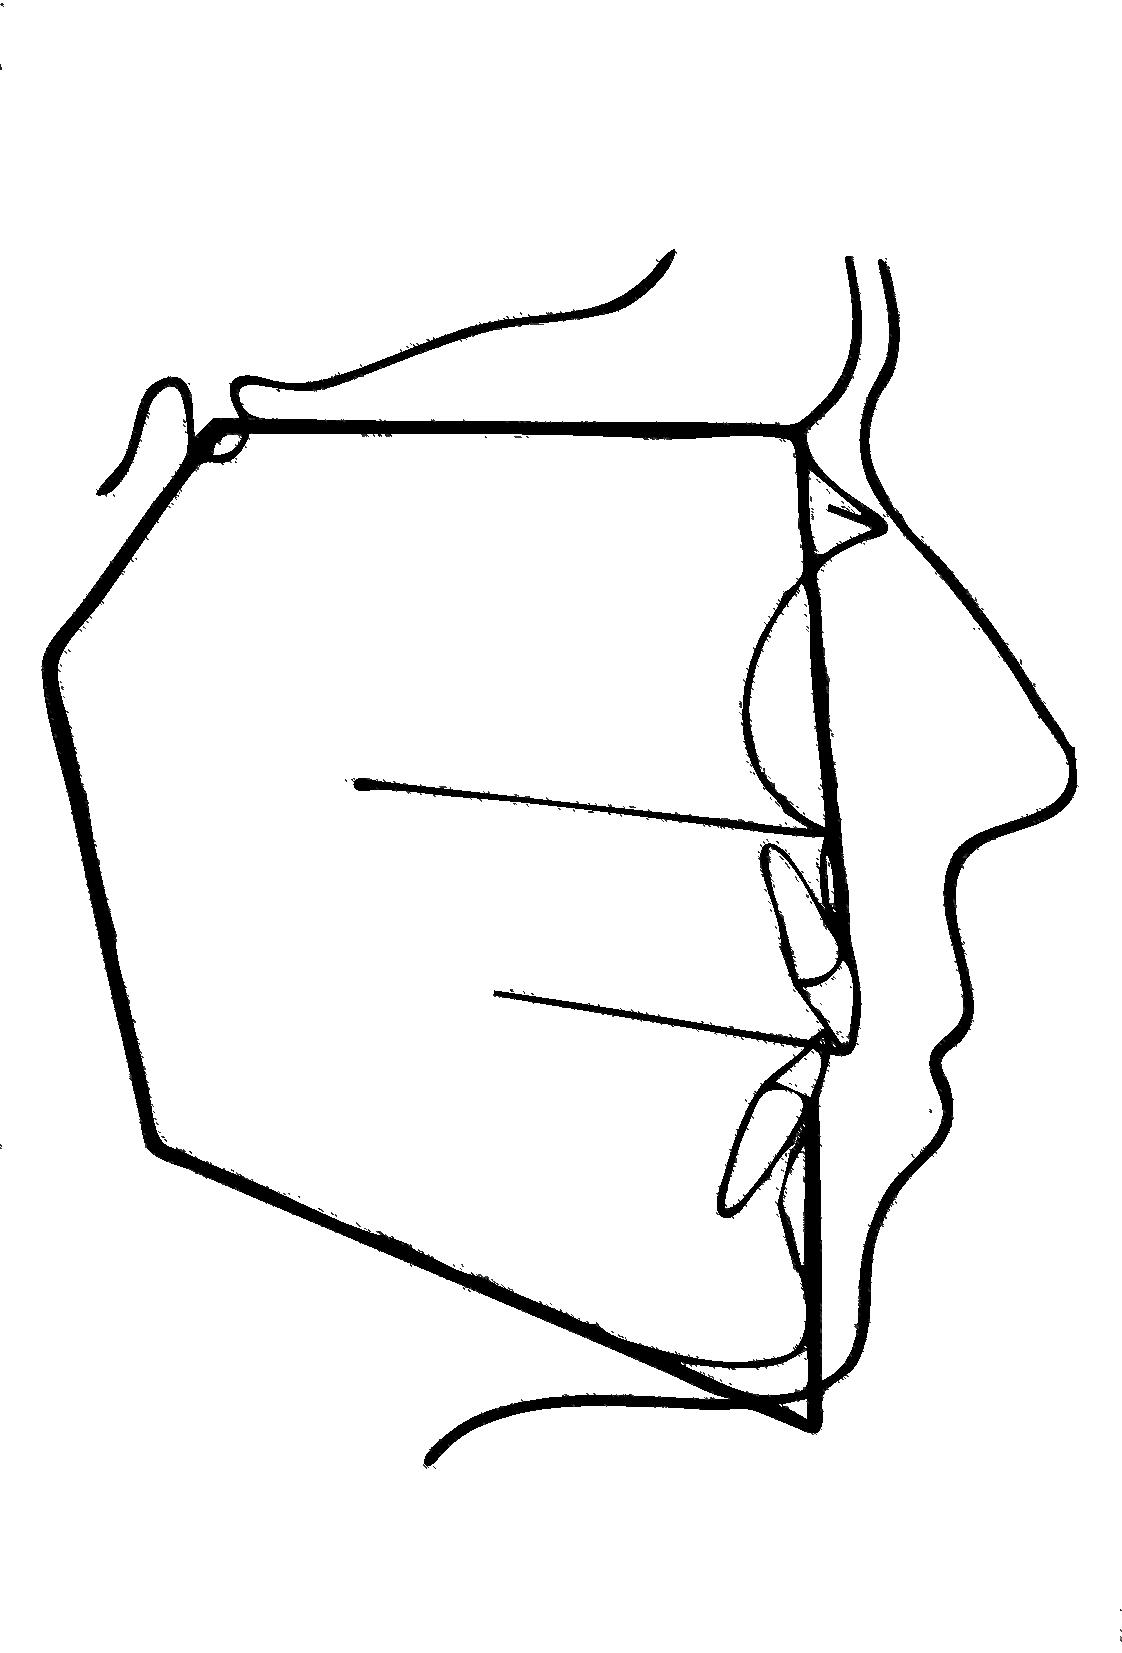
\includegraphics[width=.3\textwidth]{./images/bjork-a.pdf}}} \quad
\subfloat[][]
   {\fbox{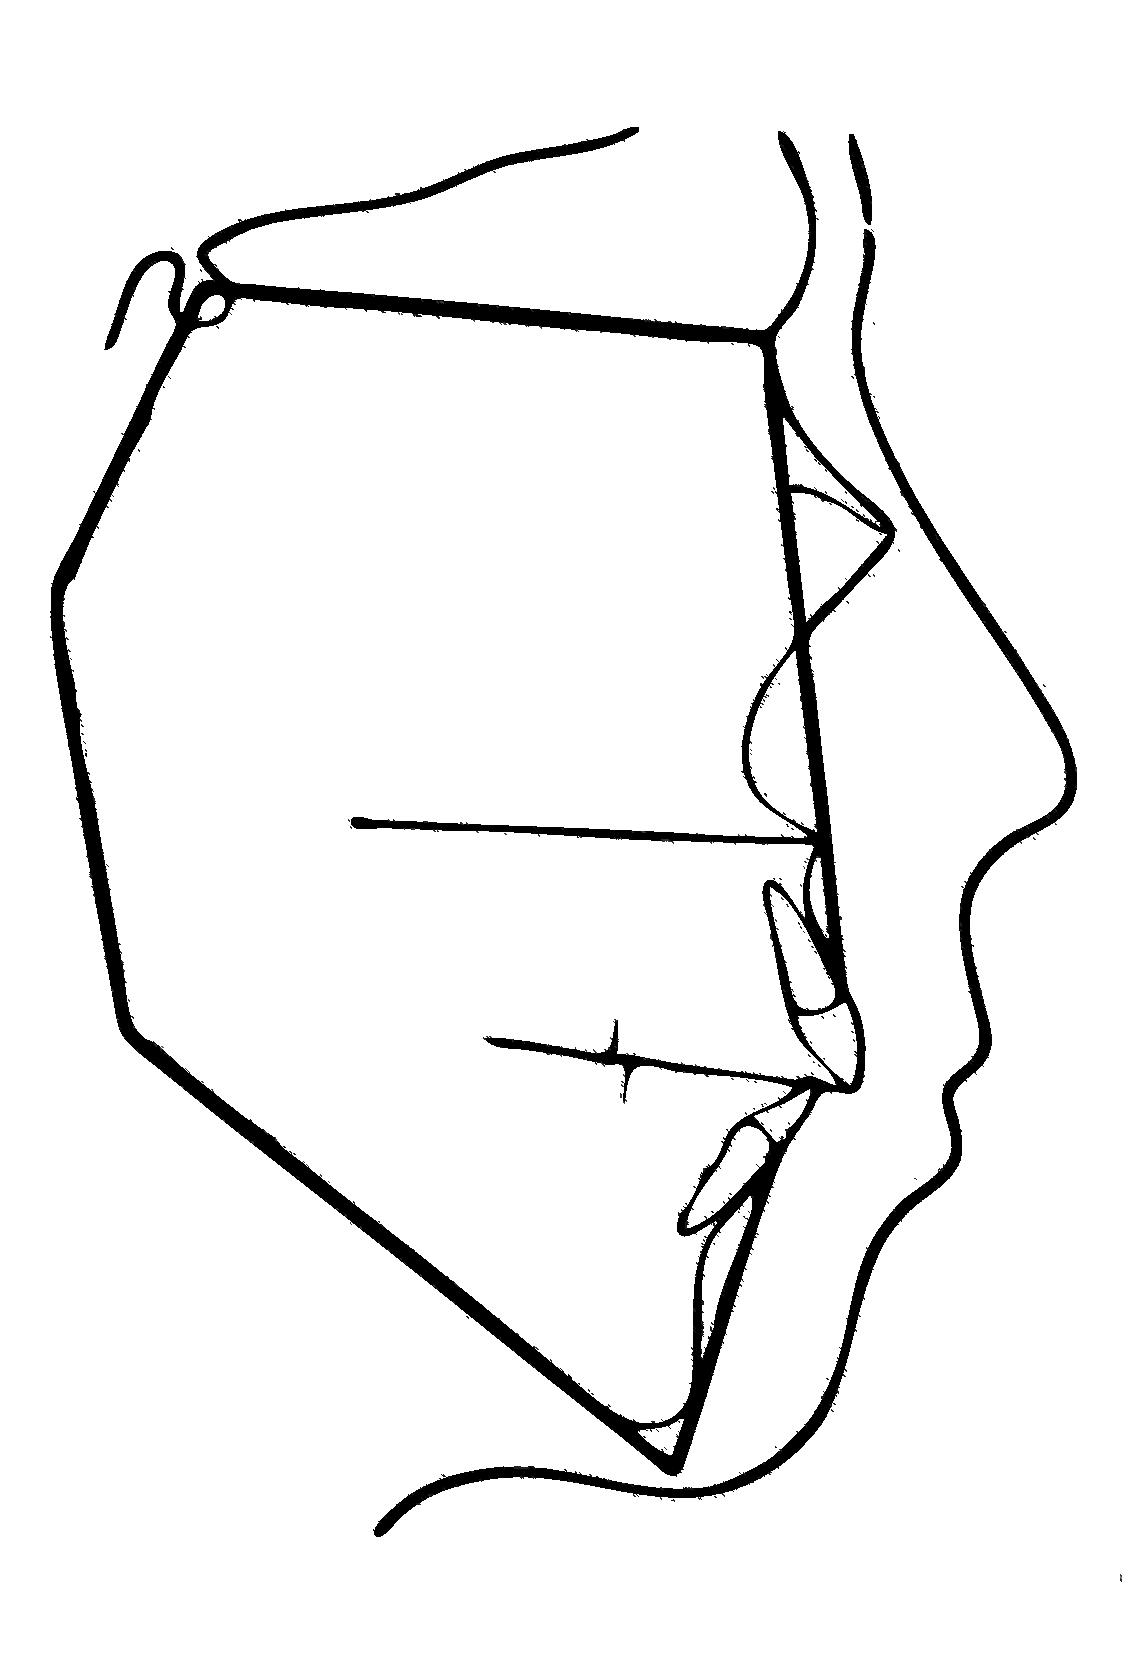
\includegraphics[width=.3\textwidth]{./images/bjork-b.pdf}}} \quad
\subfloat[][]
   {\fbox{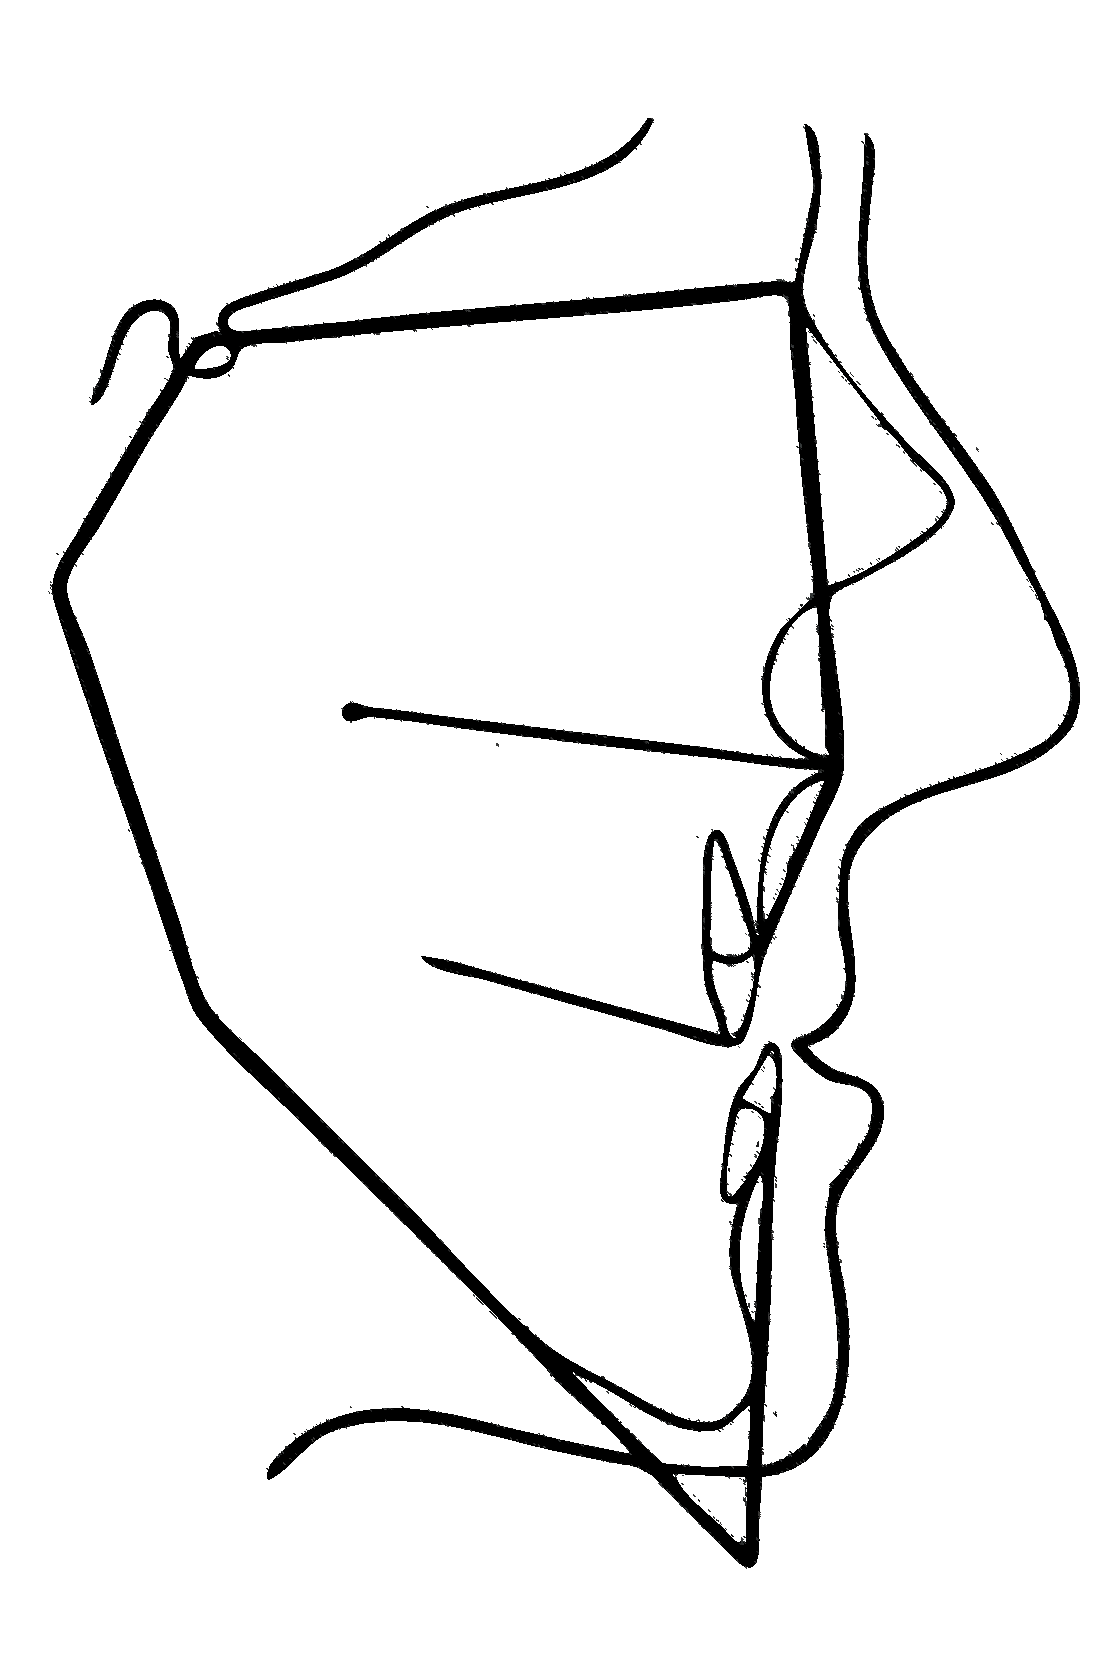
\includegraphics[width=.3\textwidth]{./images/bjork-c.pdf}}}
\caption{Studi di Björk sui profili facciali.}
\label{fig:bjork-profili}
\end{figure}

\subsection{Il ventesimo secolo}
L'evoluzione della cefalometria nel ventesimo secolo è universalmente collegata alla pubblicazione di Edward Angle sulle malocclusioni\footcite{Angle1899}, nel 1899. Angle usava le relazioni tra l'arcata superiore ed inferiore, esemplificata dall'intercuspidazione dei primi molari permanenti, come la base per caratterizzare i tipi di malocclusione.

\begin{SCfigure}[][!t]
\centering
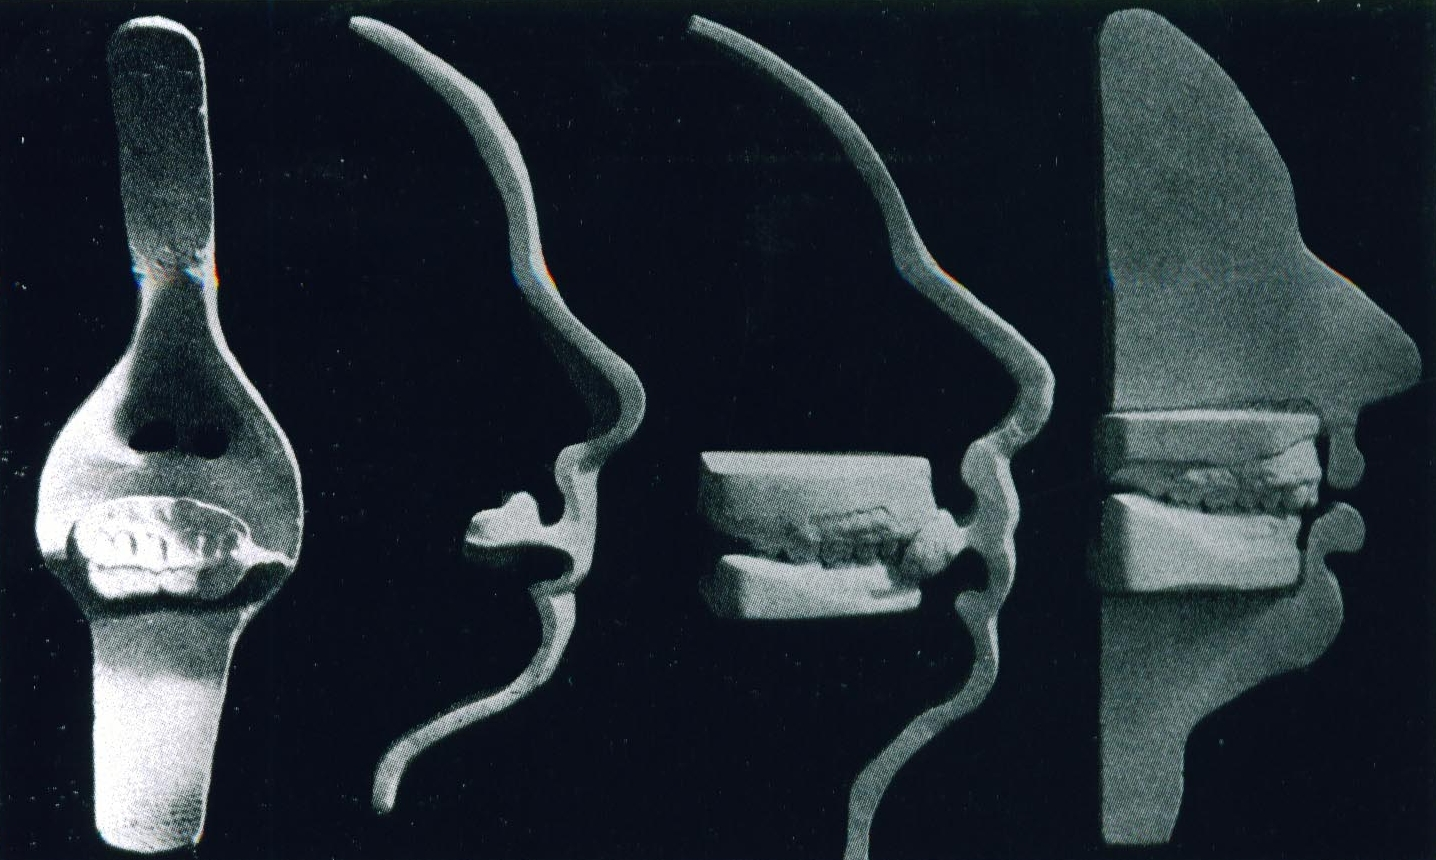
\includegraphics[width=.7\textwidth]{./images/vanloon.jpg}
% vanloon.jpg: 1436x860 pixel, 72dpi, 50.66x30.34 cm, bb=0 0 1436 860
\caption{van Loon costruì un modello tridimensionale del profilo facciale, per poter meglio studiare i rapporti tra quest'ultimo e la dentatura del paziente.}
\label{fig:vanloon}
\end{SCfigure}

Un avanzamento concettuale in senso realistico fu fatto nel 1915 da van Loon, che determinò che per una diagnosi e un piano di trattamento significativi era necessario un sistema tridimensionale che potesse determinare la relazione della dentatura con la faccia. Egli sviluppò quindi un metodo con cui la dentatura e la faccia potessero essere studiati sia separatamente, sia in relazione l'uno con l'altro. Il metodo consisteva nel prendere un'impronta parziale del profilo (fronte, naso, labbra, mento), e delle superfici labiali degli incisivi centrali superiori -- quest'ultimi sarebbero serviti come chiave per il posizionamento del modello delle arcate dentarie. Questa ``maschera facciale'' (fig.~\vref{fig:vanloon}) veniva poi posizionata su un supporto all'interno di un ``cubo cranioforo''. Questo era uno strumento utilizzato dagli antropologi per studiare i crani orientati secondo il piano di Francoforte. Sebbene questa procedura fosse complessa, lunga e poco pratica, è da segnalare in quanto rappresenta un passo evolutivo verso il posizionamento dei modelli dentari orientati tridimensionalmente nello spazio.

\begin{wrapfigure}{R}{.5\textwidth}
\centering
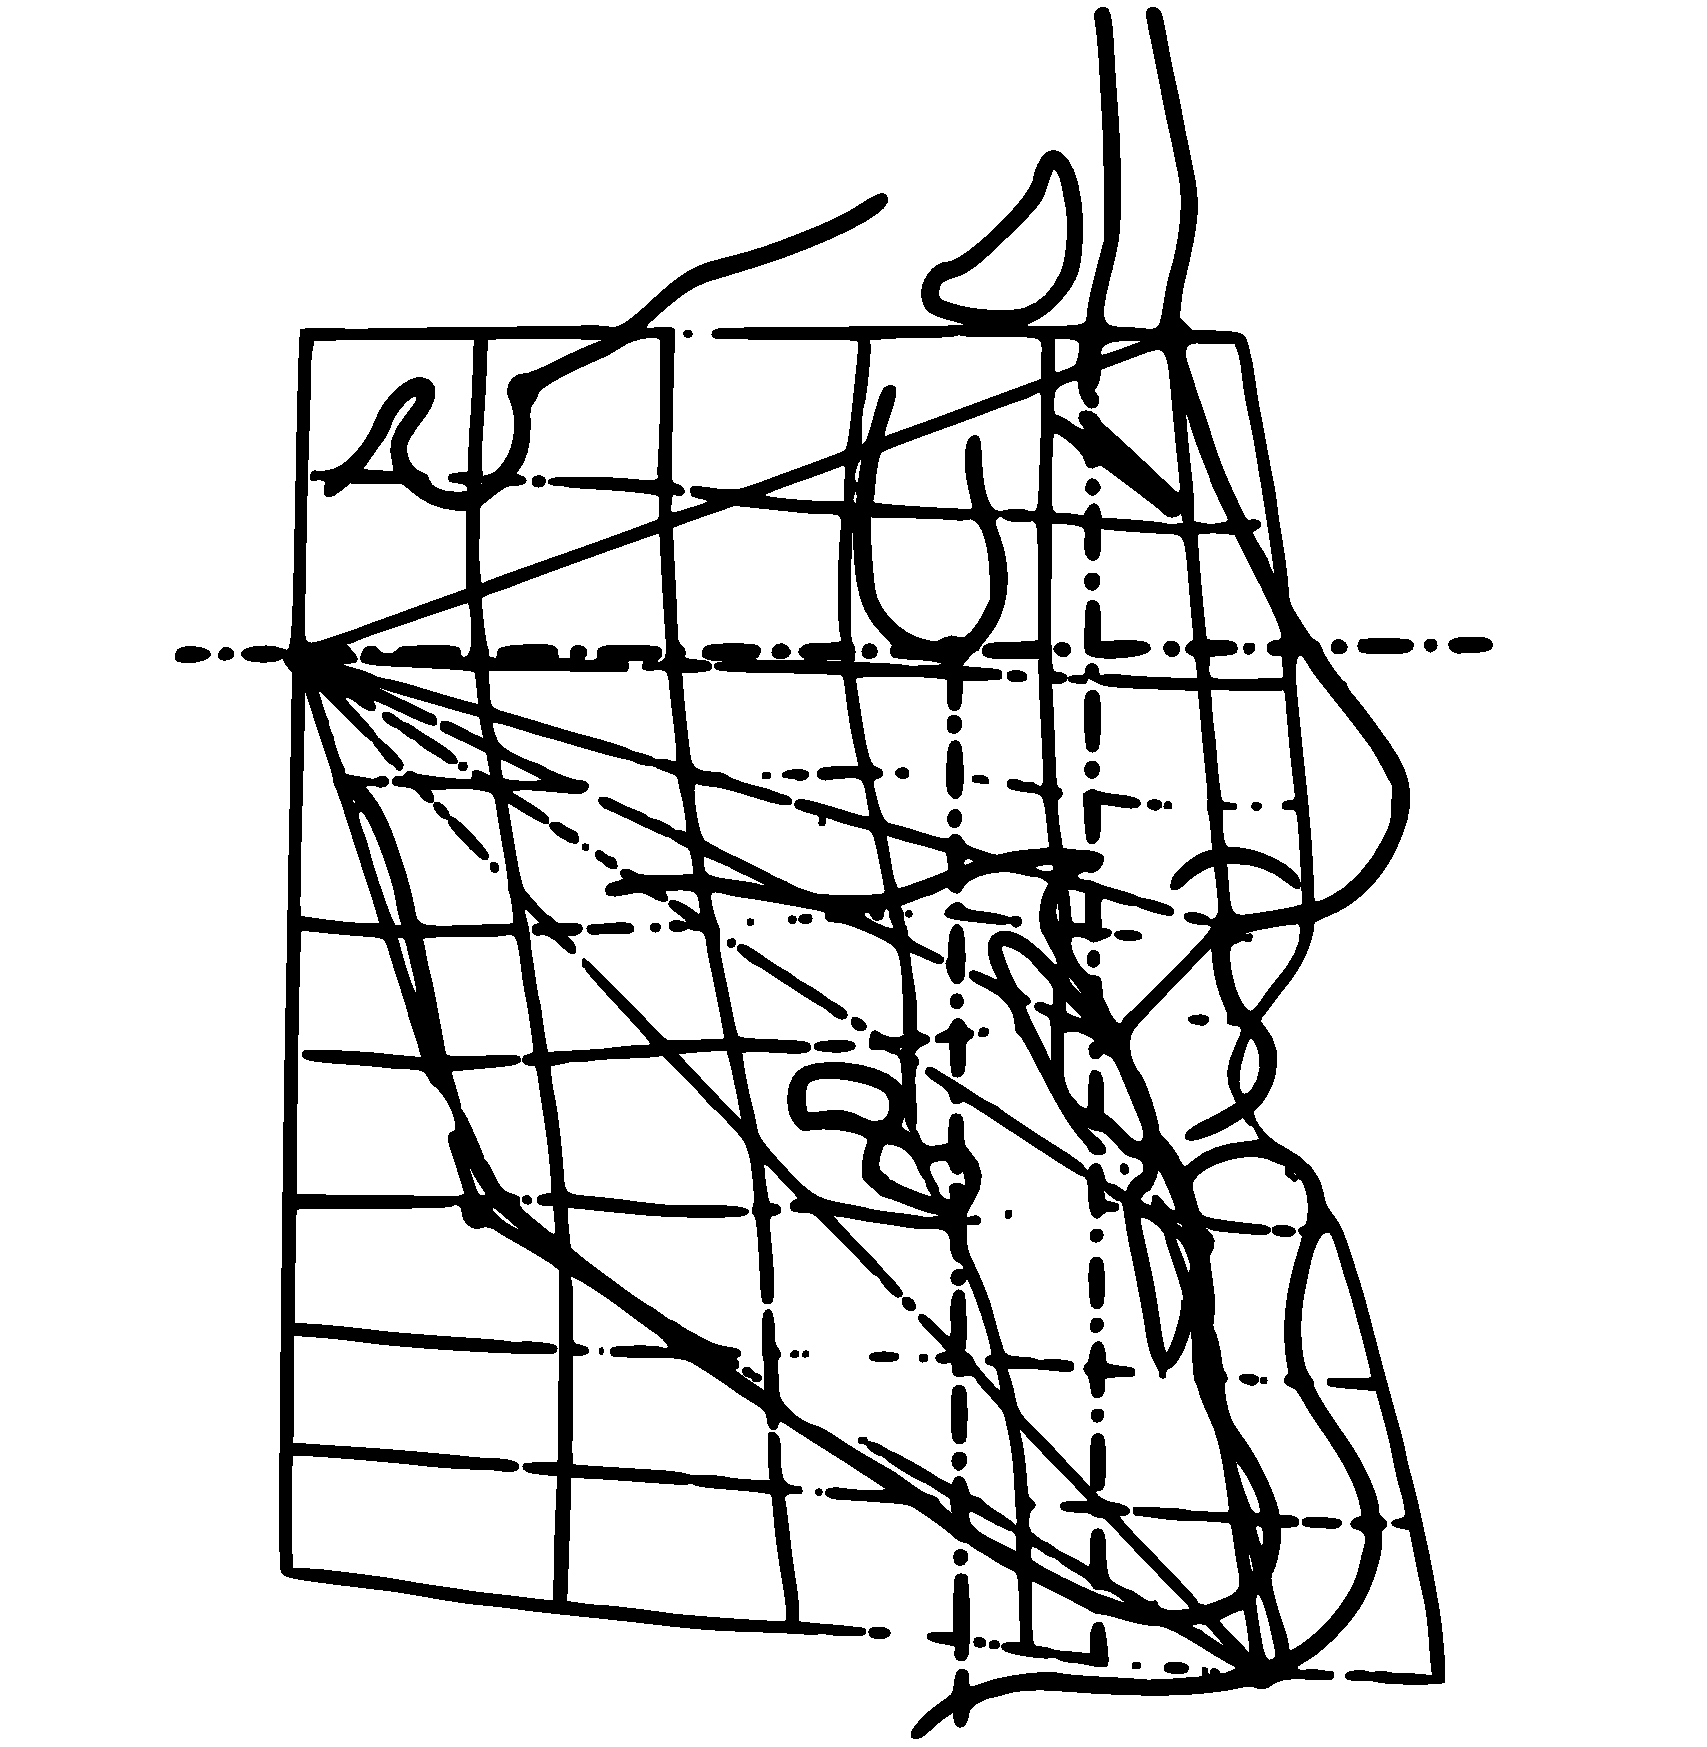
\includegraphics[width=.45\textwidth]{./images/decoster.pdf}
% decoster.pdf: 819x838 pixel, 72dpi, 28.89x29.56 cm, bb=0 0 819 838
\caption{De Coster: analisi di un individuo con marcato prognatismo mandibolare e severa malocclusione di Classe III.}
\label{fig:decoster}
\end{wrapfigure}

In seguito alla standardizzazione della radiografia cefalometrica agli inizi del 1900, Lucien de Coster\footcite{Coster1939} fu il primo a pubblicare un'analisi basata sulle relazioni di proporzionalità usate nell'antichità (fig.~\vref{fig:decoster}). De Coster utilizzò le distorsioni di un sistema di coordinate Cartesiano per mostrare le differenze di posizione dei marker in confronto alla norma\footcite{Izard1943}.

\section{La divina proporzione}

Fin dai primi dati disponibili, i ritratti del corpo umano sono stati guidati da sistemi di proporzionalità tra le sue parti. Questa procedura consentiva la riproduzione di relazioni armoniose tra le caratteristiche facciali e il resto del corpo.

\begin{wrapfigure}{R}{.5\textwidth}
\centering
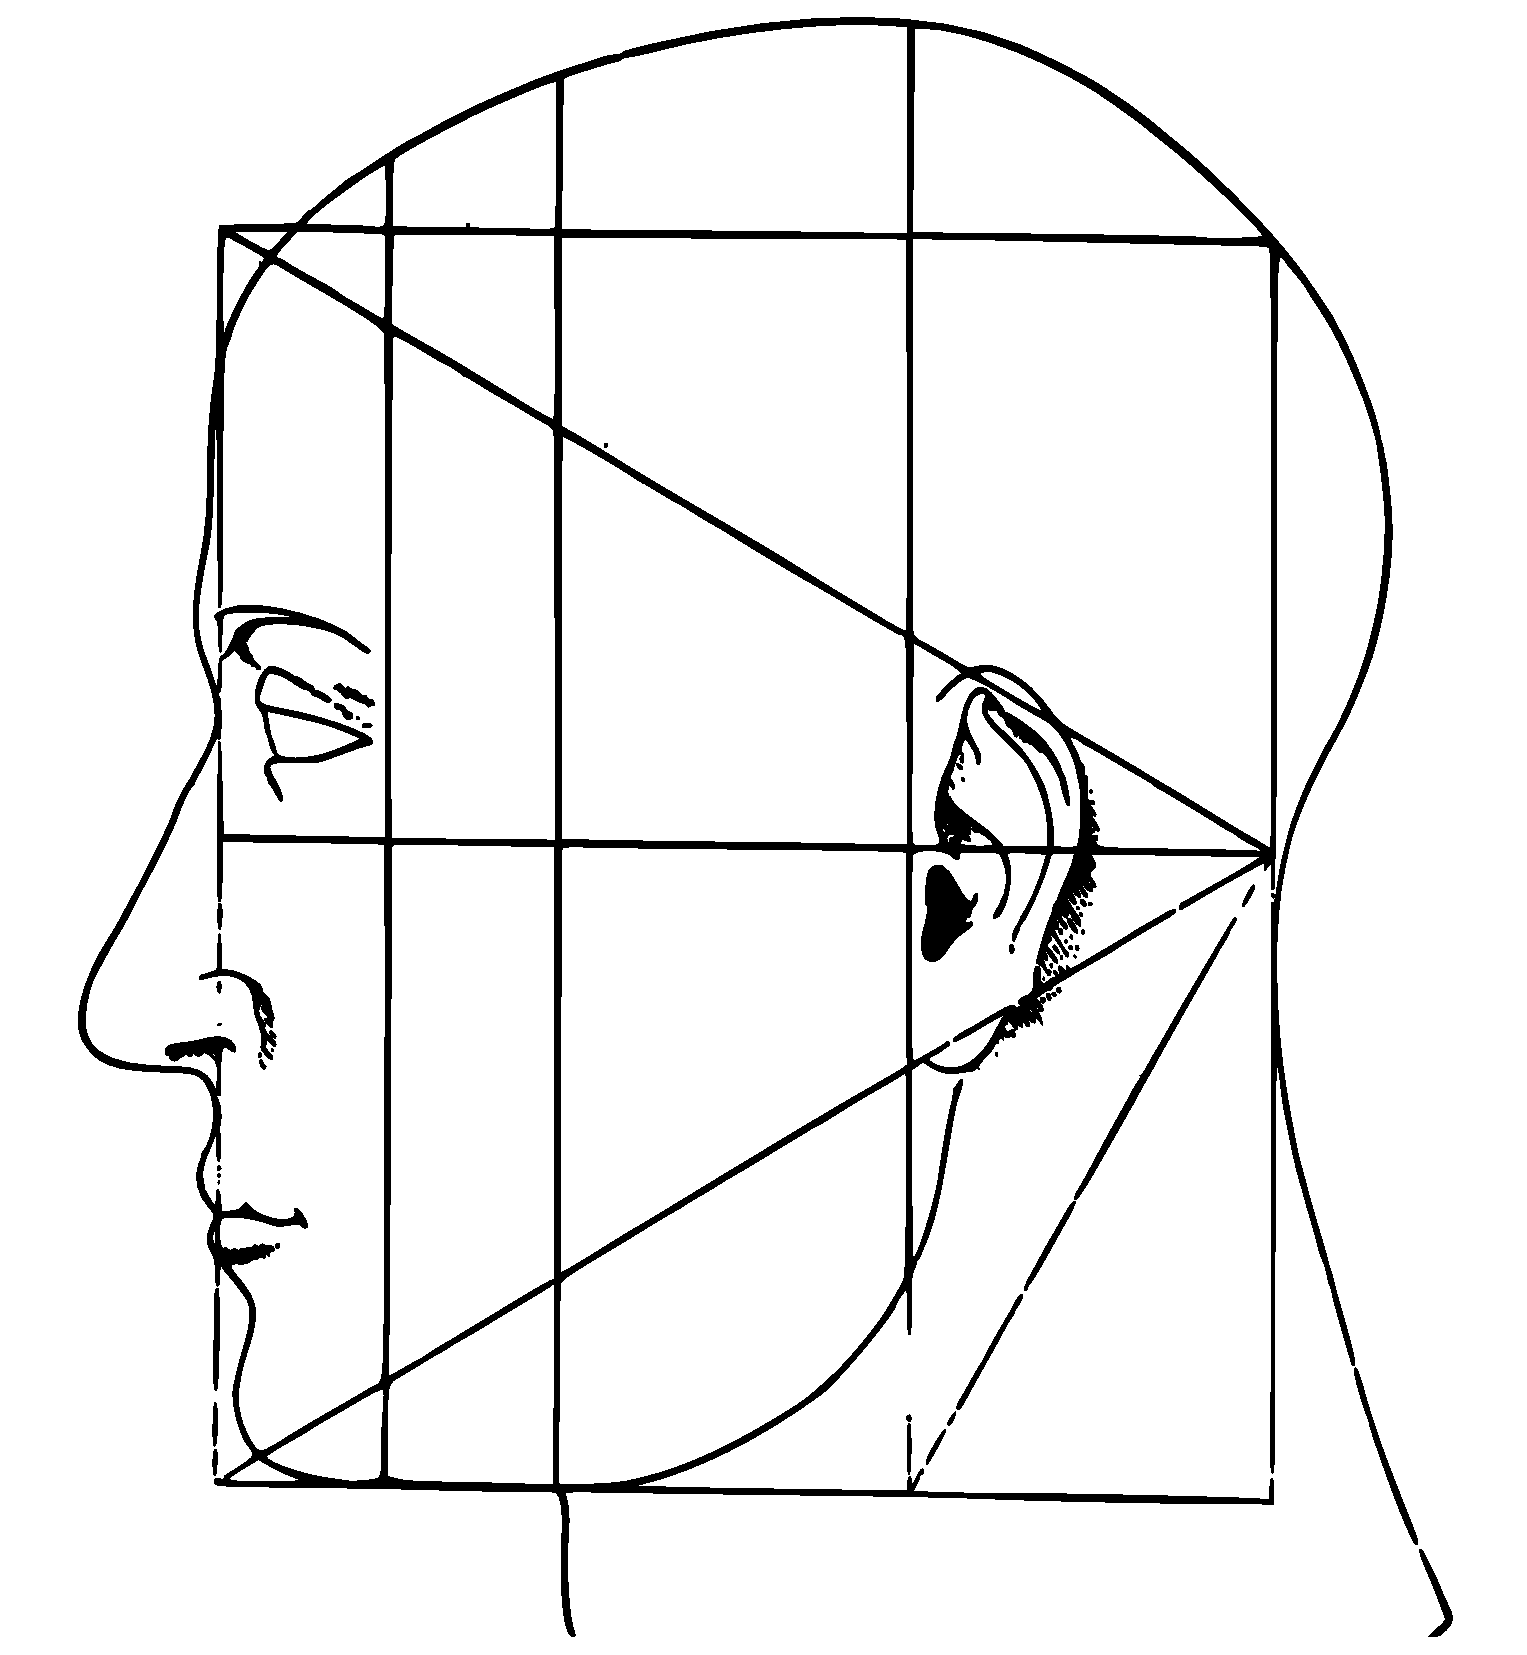
\includegraphics[width=.45\textwidth]{./images/pacioli.pdf}
% pacioli.pdf: 733x794 pixel, 72dpi, 25.86x28.01 cm, bb=0 0 733 794
\caption{Nel 1509, fra' Luca Pacioli, nella sua presentazione sulla divina proporzione, mostrò un'illustrazione di un profilo umano inquadrato in un triangolo ed un rettangolo aureo.}
\label{fig:pacioli}
\end{wrapfigure}

Nella \textit{sezione aurea} (la ``\textit{divina proporzione}''), sviluppata dagli antichi matematici Greci, la lunghezza di una linea è divisa in due parti tali che la parte minore, divisa per la parte maggiore, è uguale alla parte maggiore divisa per la lunghezza totale. Oltre ad avere applicazioni matematiche, la sezione aurea costituisce un ideale per le valutazioni di natura estetica.

Nel 1509, Luca Pacioli\footcite{Pacioli1509}, presentò un'orazione sulla sezione aurea in ambito matematico. La sua pubblicazione conteneva un disegno di un profilo umano, inquadrato in un triangolo ed un rettangolo aureo (fig.~\vref{fig:pacioli}).

Nella progettazione del volto umano, la Natura ha evidentemente trasposto la \textit{divina proporzione} in una sequenza di relazioni armoniose tra i tessuti molli e i tessuti duri. %Paradies\footnote{biblio 40} ha dimostrato che la sezione aurea è la chiave per determinare l'altezza facciale inferiore nella riabilitazione di pazienti edentuli.

Ricketts\footcite{Ricketts1982,Ricketts1982a} fu il primo, nella storia recente, ad esporre in dettaglio sulla relazione tra la struttura e la crescita della faccia e la divina proporzione e la serie di Fibonacci.
